\chapter{Theoretische Grundlagen}\label{chap_foundation}
In den folgenden Abschnitten wird der \emph{Explorationsprozess} und dessen Grundlagen formal beschrieben sowie zum besseren Verständnis mit entsprechenden Beispielen untermalt. Die einzelnen Schritte des Prozesses finden sich damit in den  Überschriften der Abschnitte wieder.

\section{Strukturelle Evaluation}
In Anlehnung an \cite{hummel08} werden die \emph{EJBs} auf der Basis des Signature-Matching Ansatzes ermittelt. Dieser Ansatz wurde ursprünglich von Zaremski und Wing \cite{moormann} beschrieben. Er basiert darauf, dass lediglich die Methoden-Signaturen der Typen (Klassen bzw. \Gls{Interface}s) miteinander abgeglichen (gematcht) werden. 
\\\\
Zu diesem Zweck wird eine Struktur zur Deklaration von Typen in Abschnitt \ref{sec:strukturTypen} vorgegeben, die eine abstrakte Darstellung von Klassen oder \Gls{Interface}s, darstellen. Darüber hinaus werden in den genannten Abschnitt die Eigenschaften der Typen sowie Funktionen vorgestellt, die für den weiteren Verlauf der Arbeit von Belang sind.
\\\\
Der Abgleich der Methoden-Signaturen dieser Typen erfolgt in Anlehnung an \cite{moormann} auf der Basis von Matchern, welche in Abschnitt \ref{sec_matcher} genauer beschrieben werden. Einige der dort beschriebenen Matcher basieren auf denen aus \cite{moormann}. Andere basieren auf Überlegungen aus \cite{hummel08}.
\subsection{Struktur für die Definition von Typen}\label{sec:strukturTypen}
Die Typen werden in einer Bibliothek $L$ wie in Tabelle \ref{tab_typeStruct} deklariert. Listing \ref{lst:libEx} zeigt die Deklaration der Bibliothek \emph{ExampLe} als Beispiel für eine Bibilothek mit \emph{required} und \emph{provided Typen}\footnote{Zu beachten ist, dass die Bibliothek auf die im JDK enthaltenen Typen aufbaut. Daher ist davon auszugehen, dass Typen wie $\texttt{Object}$ oder $\texttt{boolean}$ bereits als \emph{provided Typen} definiert sind.}.
\\\\
Zudem sei die Relation $<$ auf Typen durch folgende Regeln definiert:
\begin{gather*}
\frac{\texttt{provided }T \texttt{ extends } T' \in L}{T < T'}
\end{gather*}
\begin{gather*}
\frac{\texttt{provided } T \texttt{ extends } T'' \in L \wedge T'' < T'}{T < T'}
\end{gather*}
\noindent

\begin{table}[h!]
\centering
\begin{tabular}{|p{4.5cm}|p{7.5cm}|}
\hline
\hline
\centering\textbf{Regel} & \textbf{Erläuterung} \\
\hline
\hline
$\mathit{L} ::= \mathit{TD}\text{*}$ & Eine Bibliothek \emph{L} besteht aus einer Menge von Typdefinitionen.\\
\hline
$\mathit{TD} ::= \mathit{PD} | \mathit{RD}$ & Eine Typdefinition kann entweder die Definition eines \emph{provided Typen} (PD) oder eines \emph{required Typen} (RD) sein.\\
\hline
$\mathit{PD} ::= \newline\texttt{provided }T \texttt{ extends } T' \newline  \texttt{\{} \mathit{FD}\text{*} \mathit{MD}\text{*}\texttt{\}}$& Die Definition eines \emph{provided Typen} besteht aus dem Namen des Typen \emph{T}, dem Namen des Super-Typs \emph{T'} von \emph{T} sowie mehreren Feld- und Methodendeklarationen.\\
\hline
$\mathit{RD} ::= \texttt{required } T \texttt{ \{}\mathit{MD}\text{*}\texttt{\}}$ & Die Definition eines \emph{required Typen} besteht aus dem Namen des Typen \emph{T} sowie mehreren Methodendeklarationen.\\
\hline
$\mathit{FD} ::= T \texttt{ }\mathit{f}$ & Eine Felddeklaration besteht aus dem Namen des Feldes \emph{f} und dem Namen seines Typs \emph{T}.\\
\hline
$\mathit{MD} ::= \mathit{T'}\texttt{ }\mathit{m(T_1,...,T_n)}$ & Eine Methodendeklaration besteht aus dem Namen der Methode \emph{m}, den insgesamt $n$ Namen der Parameter-Typen $T_1$ bis $T_n$ und dem Namen des Rückgabe-Typs \emph{T'}.\\
\hline
\hline
\end{tabular}
\caption{Struktur für die Definition einer Bibliothek von Typen}
 \label{tab_typeStruct}
\end{table}
\noindent
Darüber hinaus seien folgende Funktionen definiert:
\begin{gather*}
\mathit{members(T)} :=  \left\{ 
				\begin{array}{l|l}
					T \texttt{ }\mathit{f} & T \texttt{ }\mathit{f}\text{ ist Felddeklaration von }T
				\end{array}
              \right\}
\\
\mathit{memType(f,T)} := 
				\begin{array}{l|l}
					T' & T' \texttt{ }\mathit{f} \in \mathit{members(T)}
				\end{array}   
\\
\mathit{ret(T'\text{ }m(T''_1,...T''_n))} := T'
\\
\mathit{params(T''\text{ }m(T'_1,...T'_n))} := \{ T'_1,...,T'_n \}
\\   
\mathit{methods(T)} := \left\{ 
				\begin{array}{l|l}
					T'' \text{ }m(T'_1,...,T'_n) 
					& 
\begin{array}{l}					
	T'' \text{ }m(T'_1,...,T'_n) \text{ ist}
	\\
	\text{Methodendeklaration von }T
	\end{array}
\end{array}
              \right\}
\\        
\end{gather*}
\noindent
\begin{multicols}{2}
\begin{lstlisting}[caption={Bibliothek \emph{ExampLe} von Typen},captionpos=b, style = dsl, label=lst:libEx]
provided Fire extends Object{}

provided FireState extends Object{
 boolean isActive
}

provided Injured extends Object{
 void heal(Medicine med)	
}

provided FireFighter extends Object{
 FireState extinguishFire(Fire fire)
}

provided InverseDoctor extends Object{	
 void heal( Medicine med, Patient pat )
}

required PatientMedicalFireFighter {
 void heal( Patient patient, 
            MedCabinet med )
 boolean extinguishFire( ExtFire fire )	
}




provided ExtFire extends Fire{}

provided Medicine extends Object{
 String getDescription()
}

provided Patient extends Injured{
 String getName()
}

provided Doctor extends Object{	
 void heal( Patient pat, Medicine med )
}

provided MedCabinet extends Object{
 Medicine med
}

required MedicalFireFighter {
 void heal( Injured injured, 
            MedCabinet med )
 boolean extinguishFire( ExtFire fire )	
}
\end{lstlisting}
\end{multicols}
\noindent

\subsection{Definition der Matcher}\label{sec_matcher}
Ein Matcher definiert das Matching eines Typs $T$ zu einem Typ $T'$ oder einer Methode $m$ zu einer Methode $m'$ durch die asymmetrische Relation $\Rightarrow$ (auch Matchingrealtion genannt)\footnote{$T \Rightarrow T'$\newline Gesprochen: $T$ matcht $T'$}. Im Folgenden werden die Matchingrelationen der spezifischen Matcher über ein Subskript differenziert.
\subsubsection{ExactTypeMatcher}\label{sec:exacttypematcher}
Der \emph{ExactTypeMatcher} definiert das Matching von einem Typ $T$ zu sich selbst her (vgl. \cite{moormann}). Die dazugehörige Matchingrelation $\Rightarrow_{exact}$ wird durch folgende Regel beschrieben:
\begin{gather*}
\frac{}{T \Rightarrow_{exact} T}
\end{gather*}
\subsubsection{GenTypeMatcher}\label{sec:gentypematcher}
Der \emph{GenTypeMatcher} definiert das Matching von einem Typ $T$ zu einem Typ $T'$ mit $T > T'$ (vgl. \cite{moormann}). Die dazugehörige Matchingrelation $\Rightarrow_{gen}$ wird durch folgende Regel beschrieben:
\begin{gather*}
\frac{T > T'}{T \Rightarrow_{gen} T'}
\end{gather*}
\subsubsection{SpecTypeMatcher}
Der \emph{SpecTypeMatcher} definiert im Verhältnis zum \emph{GenTypeMatcher} das Matching in die entgegengesetzte Richtung (vgl. \cite{moormann}). Die dazugehörige Matchingrelation $\Rightarrow_{spec}$ wird durch folgende Regel beschrieben: 
\begin{gather*}
\frac{T < T'}{T \Rightarrow_{spec} T'}
\end{gather*}
\noindent
Die oben genannten Matchingrelationen werden für die Definition weiterer Matcher zusammengefasst, wodurch sich die Matchingrelation $\Rightarrow_{internCont}$ ergibt:
\begin{gather*}
\frac{T \Rightarrow_{exact} T' \vee T \Rightarrow_{gen} T' \vee
T \Rightarrow_{spec} T'  }{T \Rightarrow_{internCont} T'}
\end{gather*}
\noindent
\\\\
Die folgenden Matcher definieren das Matching für so genannte \Gls{wrappertype}en zu den Typen der in ihnen enthaltenen Attribute. Die Idee für solche Matcher fand in \cite{hummel08} zwar Erwähnung, jedoch erfolgte dort keine formale Beschreibung. Das Ziel dieser Matcher ist es bspw. die Typen $\texttt{boolean}$ und $\texttt{FireState}$ aus der in Listing \ref{lst:libEx} deklarierten Bibliothek zu matchen.
\subsubsection{ContentTypeMatcher}
Der \emph{ContentTypeMatcher} definiert das Matching von einem Typ $T$ zu einem Typ $T'$, wobei $T'$ ein Feld enthält, auf dessen Typ $T''$ der Typ $T$ über die Matchingrelation $\Rightarrow_{internCont}$ gematcht werden kann.
\\\\
Die dazugehörige Matchingrelation $\Rightarrow_{content}$ wird durch folgende Regel beschrieben:
\begin{gather*}
\frac{\exists \mathit{T''\text{ }f}\in members(T'): T \Rightarrow_{internCont} T''}{T \Rightarrow_{content} T'}
\end{gather*}
\noindent
So würde für die Typen $\texttt{boolean}$ und $\texttt{FireState}$ aus der Bibliothek \emph{ExampLe} (siehe Listing \ref{lst:libEx}) gelten: 
\begin{gather*}
\texttt{boolean} \Rightarrow_{content} \texttt{FireState}
\end{gather*}
\subsubsection{ContainerTypeMatcher}
Der \emph{ContainerTypeMatcher} definiert im Verhältnis zum \emph{ContentTypeMatcher} das Matching für die entgegengesetzte Richtung.
\\\\
Die dazugehörige Matchingrelation $\Rightarrow_{container}$ wird durch folgende Regel beschrieben:
\begin{gather*}
\frac{\exists \mathit{T''\text{ }f}\in members(T): T'' \Rightarrow_{internCont} T'}{T \Rightarrow_{container} T'}
\end{gather*}
\noindent
So gilt für die Typen $\texttt{FireState}$ und $\texttt{boolean}$ aus der Bibliothek \emph{ExampLe} (siehe Listing \ref{lst:libEx}): 
\begin{gather*}
\texttt{FireState} \Rightarrow_{container} \texttt{boolean}
\end{gather*}
\\\\
Zur Definition des letzten Matchers werden die Matchingrelationen der oben genannten Matcher wiederum zusammengefasst. Dabei entsteht die Matchingrelation $\Rightarrow_{internStruct}$, welche durch folgende Regel beschrieben wird:
\begin{gather*}
\frac{T \Rightarrow_{internCont}T' \vee T \Rightarrow_{container} T' \vee T \Rightarrow_{content} T'}{T \Rightarrow_{internStruct}T'}
\end{gather*}
\subsubsection{StructuralTypeMatcher} \label{subsec_structmatcher}
Der \emph{StructuralTypeMatcher} definiert das Matching von einem \emph{required Typ} $R$ zu einem \emph{provided Typ} $T$ auf der Basis der Methoden-Signaturen der beiden Typen.
\\\\
Somit soll bspw. ein Matching zwischen dem Typ $\texttt{MedicalFireFighter}$ und dem den $\texttt{FireFighter}$ aus der Bibliothek \emph{ExampLe}  (siehe Listing \ref{lst:libEx}) gematcht werden. Als ein weiteres Beispiel, bezogen auf die Typen aus der Bibliothek \emph{ExampLe}, kann das Matching zwischen dem Typ $\texttt{MedicalFireFighter}$ und dem Typ $\texttt{Doctor}$ angebracht werden.
\\\\
Damit ein \emph{required Typ} $R$ auf einen \emph{provided Typ} $T$ über den \emph{StrukturalTypeMatcher} gematcht werden kann, muss mindestens eine Methode aus $R$ zu einer Methode aus $T$ gematcht werden (Signature-Matching). Ein Matching der Methoden liegt dann vor, wenn sowohl die Rückgabe- als auch die Parameter-Typen dieser beiden Methoden miteinander gematcht werden können (vgl. \cite{moormann}). 
\\\\
Wie in \cite{moormann} soll die Reihenfolge, in der die Parameter in der jeweiligen Methode deklariert wurden, keine Rolle spielen. Ausgehend von den Parameter-Typen der beiden Methoden als Mengen, muss eine der Mengen also so umsortiert werden, dass die Parameter-Typen aus beiden Mengen an der jeweils gleichen Position miteinander gematcht werden können.
Die möglichen umsortierten Mengen von Parameter-Typen einer Methode $m$ auf die dies in Bezug auf die Menge der Parameter-Typen einer Methode $m'$ zutrifft, werden über die Funktion $\mathit{matchingParams}$ beschrieben:
\begin{gather*}
\mathit{matchingParams(m, m')} :=
\left\{
\begin{array}{l|l}
	\left\{
	\begin{array}{l}
		 \mathit{P'_1},\\
		 \mathit{...,} \\
		 \mathit{P'_n}
	\end{array}
	\right\}
	&
	\begin{array}{l}
		\{\mathit{P_1,...,P_n}\} = \mathit{params(m)} 				\wedge \mathit{ }
		\\
		\forall i \in \{1,...,n\}: \mathit{P'_i} \in 				\mathit{params(m'}) \wedge \mathit{ }
		\\	
		\mathit{P'_i} \Rightarrow_{internStruct} 					\mathit{P_i}
	\end{array}
\end{array}
\right\}
\end{gather*}
\noindent
Das Matching zweier Methoden $m$ und $m'$ wird durch die Relation $\Rightarrow_{method}$ über folgende Regel beschrieben:
\begin{gather*}
\frac{\mathit{ret(m)} \Rightarrow_{internStruct} \mathit{ret(m')} \wedge \mathit{matchingParams(m,m')} \neq \emptyset}{m \Rightarrow_{method} m'}
\end{gather*}
\noindent
Die Menge der gematchten Methoden aus $R$ in $T$ wird darauf aufbauend durch folgende Funktion beschrieben:
\begin{gather*}
structM_{source}(R,T) := \left\{ 
				\begin{array}{l|l}
m	& \mathit{m} \in \mathit{methods(R)} \wedge \mathit{ }
\\
	& \exists \mathit{m'} \in \mathit{methods(P)} : m \Rightarrow_{method} m'
				\end{array}
              \right\}
\end{gather*}
\noindent
Die Matchingrelation für den \emph{StructuralTypeMatcher} wird durch folgende Regel beschrieben:
\begin{gather*}
\frac{structM_{source}(R,T) \neq \emptyset}{R \Rightarrow_{struct}T}
\end{gather*}


\subsection{Ergebnis der strukturellen Evaluation}\label{sec_ergStructEval}
Die Exploration wird für einen \emph{required Typ} durchgeführt. Bei der \emph{strukturellen Evaluation} sollen Mengen von \emph{provided Typen} ermittelt werden, deren Methoden in Kombination zu jeder Methode des \emph{required Typ} ein Matching aufweisen. Die Mengen von \emph{provided Typen} innerhalb einer Bibliothek $L$ für die dies in Bezug auf ein \emph{required Typ} $R$ zutrifft, wird über die Funktion $cover$ beschrieben.
\begin{gather*}
cover(R,L) := 
\left\{\begin{array}{l|l}
					& T_1 \in L \wedge \text{...} \wedge T_n \in L 								\wedge \mathit{ }\\
\{T_1,...,T_n\}		& \mathit{methods(R)} = \mathit{structM(R,T_1)}							\cup \mathit{ }\\
					& \texttt{...} \cup \mathit{structM(R, T_n)} 								\wedge \mathit{ }\\
					& \forall T \in \{T_1,...,T_n\}:											\mathit{structM(R,T)} \neq \emptyset
\end{array}\right\}
\end{gather*}
Die \emph{provided Typen} innerhalb dieser Mengen werden im nächsten Schritt des \emph{Explorationsprozesses} als \emph{Target-Typen} bezeichnet und als Basis für die Generierung der Proxies für den \emph{required Typ} $R$ verwendet.
\newpage
\begin{example}{bsp_cover}
Sei folgende Bibliothek $L$ gegeben.
\begin{lstlisting}[style = dsl]
provided Come extends Object{
 String hello()
 String goodMorning()
}

provided Leave extends Object{
 String bye()
}

required Greeting{
 String hello()
 String bye()
}
\end{lstlisting}
Über die Funktion $\mathit{cover}$ werden folgende \emph{Target-Typen} für die Generierung von Proxies für den \emph{required Typ} $\texttt{Greeting}$ ermittelt.
\begin{gather*}
\mathit{cover(\texttt{Greeting},L)} = \{
	\{\texttt{Come}\},\{\texttt{Leave}, \texttt{Come}\}
\}
\end{gather*}
\end{example}
\newpage




\section{Generierung der Proxies auf Basis von Matchern}
%TODO verknüpfung ergänzen
Ein Proxy wird in Abhängigkeit vom Matching zwischen dem Source- und den Target-Typen erzeugt. Im Folgenden werden zuerst die Matcher beschrieben. Im Anschluss wird auf die Generierung der Proxies eingegangen.
\subsection{Struktur für die Definition von Proxies}\label{sec:proxygram}
Die Konvertierung eines Typs $T$ aus einer Menge von provided Typen $P$ wird durch \emph{Proxies} beschrieben. Die Grammatikregeln für einen Proxies sind Tabelle \ref{tab:grProxies} zu entnehmen.
\begin{table}[H]
\centering
\begin{tabular}{|p{5cm}|p{9cm}|}
\hline
\hline
\centering\textbf{Regel} & \textbf{Erläuterung} \\
\hline
\hline
$\mathit{PROXY} ::=$\newline
$\texttt{proxy } \texttt{for } T$\newline
$ \texttt{with [}\mathit{P_1},...,\mathit{P_n}\texttt{]}$ \newline
$\texttt{\{}\mathit{MDEL_1},...,\mathit{MDEL_k} \texttt{\}}$
 & Ein Proxy wird für ein Typ $T$ als Source-Typ mit einer Mengen von provided Typen $P = \{P_1,...,P_n\}$ als Target-Typen, einer Menge von Methoden-Delegationen erzeugt.\\
\hline
$\mathit{MDEL} ::=$\newline
$CALLM \rightarrow DELM $  & Eine \emph{Methodendelegation} besteht aus einer \emph{aufgerufenen Methode} und aus einem \emph{Delegationsziel}.\\
\hline
$\mathit{CALLM} ::=$\newline 
$\mathit{REF}.\mathit{m(\mathit{CP_1},...,\mathit{CP_n}):CR} $  & Eine aufgerufene Methode besteht aus dem Namen der Methode $m$, dem Rückgabetyp $\mathit{CR}$ und einer Menge von Parametertypen $\{\mathit{CP_1},...,\mathit{CP_n}\}$.\\
\hline
$\mathit{DELM} ::=$\newline 
$\mathit{REF}.\mathit{n(\mathit{DP_1},...,\mathit{DP_n}):DR} $  
& Die erste Variante eines Delegationsziels besteht aus  dem Namen der \emph{Delegationsmethode} $n$, dem Rückgabetyp $\mathit{DR}$ und einer Menge von Parametertypen $\{\mathit{DP_1},...,\mathit{DP_n}\}$.\\
\hline
$\mathit{DELM} ::=$\newline
$\texttt{posModi(} \mathit{I_1},...,\mathit{I_n} \texttt{)}$\newline
$\mathit{REF}.\mathit{n(\mathit{DP_1},...,\mathit{DP_n}):DR} $  
& Die zweite Variante eines Delegationsziels besteht aus einer Menge von Indizies $\{\mathit{I_1},...,\mathit{I_n}\}$, einer \emph{Referenz}, dem Namen der Delegationsmethode $n$, dem Rückgabetyp $\mathit{DR}$ und einer Menge von Parametertypen $\{\mathit{DP_1},...,\mathit{DP_n}\}$.\\
\hline
$\mathit{DELM} ::= \texttt{err} $  
& Die dritte Variante eines Delegationsziels enthält keine weiteren Bestandteile. Das Terminal $\texttt{err}$ weist darauf hin, dass die Delegation innerhalb des Proxies nicht möglich ist und zu einem Fehler führt.\\
\hline
$\mathit{REF} ::= \mathit{P_i}$
& Die erste Variante einer Referenz besteht aus einem Typ $P_i$ .\\
\hline
$\mathit{REF} ::= \mathit{P_i}\texttt{.}\mathit{f}$
& Die zweite Variante einer Referenz besteht aus einem Typ $P_i$ und einem Feldnamen $f$.\\
\hline
\end{tabular}
\caption{Grammatikregeln mit Erläuterungen für die Definition eines Proxies}
 \label{tab:grProxies}
\end{table}
\noindent
Es handelt sich dabei um Produktionsregeln einer Attributgrammatik. Die dazugehörigen Attribute sind der Tabelle \ref{tab:attrGrProxies} zu entnehmen. Dazu sei zusätzlich festgelegt, dass die Notation $\mathit{NT}\texttt{.}\text{*}$ in der Spalte \emph{Attribute} eine Key-Value-Liste aller Attribute des Nonterminals $\mathit{NT}$ beschreibt, wobei der Attributname als Key und dessen Wert als Value innerhalb der Liste verwendet wird. Weiterhin sei ein Attribut, dass in der Spalte \emph{Attribute} zu einem Nonterminal nicht aufgeführt ist, wird mit dem Wert \emph{none} belegt.
\begin{table}[h!]
\centering
\begin{tabular}{|p{6cm}|p{8cm}|}
\hline
\hline
\centering\textbf{Regel} & \textbf{Attribute} \\
\hline
\hline
$\mathit{PROXY} ::=$\newline
$\texttt{proxy } \texttt{for } T$\newline
$ \texttt{with [}\mathit{P_1},...,\mathit{P_n}\texttt{]}$ \newline
$\texttt{\{}\mathit{MDEL_1},...,\mathit{MDEL_k} \texttt{\}}$
& 
$\texttt{type} = \mathit{T}$\newline
$\texttt{targets} = [\mathit{P_1},...,\mathit{P_n}]$\newline
$\texttt{dels} = [\mathit{MDEL_1}\texttt{.}\text{*},...,\mathit{MDEL_k}\texttt{.}\text{*}]$
\\
\hline
$\mathit{MDEL} ::=$\newline
$\mathit{CALLM} \rightarrow \mathit{DELM} $  
& 
$\texttt{call} = \mathit{CALLM}.*$\newline
$\texttt{del} = \mathit{DELM}.*$
\\
\hline
$\mathit{CALLM} ::=$\newline 
$\mathit{REF}.\mathit{m(\mathit{CP_1},...,\mathit{CP_n}):CR}$
& 
$\texttt{source} = \mathit{REF.\texttt{mainType}}$\newline
$\texttt{delType} = \mathit{REF.\texttt{delType}}$\newline
$\texttt{name} = \mathit{m}$\newline
$\texttt{paramTypes} = \mathit{[CP_1},...,\mathit{CP_n]}$\newline
$\texttt{returnType} = \mathit{CR}$\newline
$\texttt{field} = \mathit{REF}\texttt{.field}$\newline
$\texttt{paramCount} = n$
\\
\hline
$\mathit{DELM} ::=$\newline 
$\mathit{REF}\texttt{.}n(\mathit{DP_1},...,\mathit{DP_n}):DR $  
&
$\texttt{target} = \mathit{REF}.\texttt{mainType}$\newline
$\texttt{delType} = \mathit{REF}.\texttt{delType}$\newline
$\texttt{posModi} = [0,...,\mathit{n}-1]$\newline
$\texttt{name} = \mathit{n}$\newline
$\texttt{paramTypes} = \mathit{[DP_1},...,\mathit{DP_n]}$\newline
$\texttt{returnType} = \mathit{DR}$\newline
$\texttt{field} = \mathit{REF}\texttt{.field}$
\\
\hline
$\mathit{DELM} ::=\texttt{posModi(} \mathit{I_1},...,\mathit{I_n} \texttt{)}$\newline
$\mathit{REF}\texttt{.}n(\mathit{DP_1},...,\mathit{DP_n}):DR $  
&
$\texttt{target} = \mathit{REF}.\texttt{mainType}$\newline
$\texttt{delType} = \mathit{REF}.\texttt{delType}$\newline
$\texttt{posModi} = \mathit{[I_1},...,\mathit{I_n]}$\newline
$\texttt{name} = \mathit{n}$\newline
$\texttt{paramTypes} = \mathit{[DP_1},...,\mathit{DP_n]}$\newline
$\texttt{returnType} = \mathit{DR}$\newline
$\texttt{field} = \mathit{REF}\texttt{.field}$
\\
\hline
$\mathit{DELM} ::= \texttt{err} $  
&
\\
\hline
$\mathit{REF} ::= \mathit{P}$
& 
$\texttt{mainType} = \mathit{P}$\newline
$\texttt{field} = \texttt{self}$\newline
$\texttt{delType} = \mathit{P}$
\\
\hline
$\mathit{REF} ::= \mathit{P}\texttt{.}\mathit{f}$
&
$\texttt{mainType} = \mathit{P}$\newline
$\texttt{field} = \mathit{f}$\newline
$\texttt{delType} = \mathit{feldTyp(f,P)}$
\\
\hline
\end{tabular}
\caption{Grammatikregeln mit Attributen für die Definition eines Proxies}
 \label{tab:attrGrProxies}
\end{table}
\noindent
Ein Proxy bietet alle Methoden des Source-Typen an. Einige dieser Methoden werden an eine Methode delegiert, die von einem der Target-Typ des Proxies angeboten wird. Eine solche Delegation wird durch eine Methoden-Delegation (siehe Nontermial $\mathit{MDEL}$) definiert.
\paragraph{Beispiel} So beschreibt die folgende Methoden-Delegation, dass die Methode $\texttt{extinguishFire}$, die vom Source-Typ $\texttt{Patient}$ - und damit auch vom Proxy - angeboten wird, an die Methoden $\texttt{heal}$, die der Target-Typ $\texttt{Injured}$ anbietet, delegiert wird.
\begin{lstlisting}[style = dsl, caption = Einfache Methoden-Delegation, captionpos = b]
	Patient.heal(Medicine):void --> Injured.heal(Medicine):void
\end{lstlisting}
\noindent
Die Delegation einer aufgerufenen Methode an ein Delegationsziel, erfolgt in drei Schritten.
\begin{enumerate}
\item Parameterübergabe\\
Dabei werden die Parameter, mit denen die vom Proxy angebotene Methode, aufgerufen wird, an die Delegationsmethode des Delegationsziels übergeben. Dabei sind zwei Dinge zu beachten. Zum Einen müssen die Typen der übergebenen Parameter zu den Typen der von der Delegationsmethode erwarteten Parameter passen. Zum Anderen muss die Reihenfolge, in der die Parameter übergeben wurden, an die erwartete Reihenfolge der Delegationsmethode angepasst werden.
\item Ausführung\\
Dieser Schritt meint die Durchführung der Delegationsmethode mit den übergeben Parametern aus Schritt 1. Dies schließt auch die Ermittlung des Rückgabewertes der Delegationsmethode ein.
\item Übergabe des Rückgabewertes\\
Ähnlich wie bei der Parameterübergabe, muss auch der Rückgabewert, der bei der Ausführung in Schritt 2 ermittelt wurde, an die aufgerufenen Methode, die vom Proxy angeboten wird, übergeben werden. Hier muss ebenfalls sichergestellt werden, dass die beiden Rückgabetypen der beiden Methoden zueinander passen.
\end{enumerate}
Die Delegation aus dem oben genannten Beispiel kann schematisch wie in Abbildung \ref{fig:DEL_heal} dargestellt werden. Die Übergabe der Parameter- und Rückgabewerte wird durch die gestrichelten Pfeile symbolisiert.
\begin{figure}[h!]
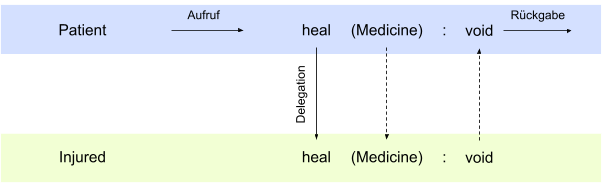
\includegraphics[width=\linewidth]{MDEL_heal}
\caption{Delegation der Methode $\texttt{heal}$}
\label{fig:DEL_heal}
\end{figure}
\noindent
An diesem Beispiel sind sowohl die Parameter- als auch die Rückgabe-Typen der aufgerufenen Methode und der Delegationsmethode identisch sind. Weiterhin spielt die Reihenfolge der Parameter in diesem Beispiel keine Rolle, da es nur einen Parameter gibt. Daher stellt die Übergabe der Parameter- und Rückgabewerte kein Problem dar.\\\\
Folgendes Beispiel soll zeigen, wie mit unterschiedlichen Reihenfolgen bzgl. der Parameter bei einer Methoden-Delegation umzugehen ist.
\paragraph{Beispiel} Die Methoden-Delegation aus Listing \ref{lst:methdel2} ist ein Beispiel für einen solchen Fall. Hier wird die aufgerufene Methode $\texttt{heal}$ mit den Parametern $\texttt{Patient}$ und $\texttt{MedCabinet}$ aus dem Typ $\texttt{PatientMedicalFireFighter}$ an die gleichnamige Methode aus dem Typ $\texttt{InverseDoctor}$ delegiert. Die Delegationsmethoden verwendet zwar identische Parameter-Typen, aber die Reihenfolge, in der die Parameter übergeben werden, ist unterschiedlich.
\begin{lstlisting}[style = dsl, caption = Methoden-Delegation mit Parametern in unterschiedlicher Reihenfolge, captionpos = b]
	PatientMedicalFireFighter.heal(Patient, MedCabinet):void --> posModi(1,0)  InverseDoctor.heal(MedCabinet,Patient):void
\end{lstlisting}\label{lst:methdel2}
\noindent
Um die Reihenfolge der Parameter aus dem ursprünglichen Aufruf zu variieren, wird das Schlüsselwort $\texttt{posModi}$ verwendet. Dort werden eine Reihe von Indizes angegeben. Die Anzahl der angegebenen Indizes muss mit der Anzahl der Parameter übereinstimmen. Ein Index beschreibt die Position des in der aufgerufenen Methode angegebenen Parameter. Weiterhin spielt die Reihenfolge der Indizes eine wichtige Rolle. Diese ist mit der Reihenfolge der Parameter der Delegationsmethoden gleichzusetzen.\\\\
So wird in dem o.g. Beispiel der erste Parameter der aufgerufenen Methoden (Index = 0) der Delegationsmethode als zweiter Parameter übergeben. Dementsprechende wird er zweite Parameter der aufgerufenen Methoden (Index = 1) der Delegationsmethode als erster Parameter übergeben (siehe Abbildung \ref{fig:DEL_healInverse}). 
\begin{figure}[H]
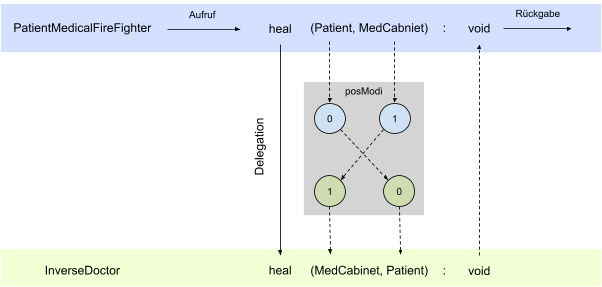
\includegraphics[width=\linewidth]{MDEL_healInverse}
\caption{Delegation der Methode $\texttt{heal}$ mit Parametern in unterschiedlicher Reihenfolge}
\label{fig:DEL_healInverse}
\end{figure}
\noindent
Ein weiteres Beispiel soll zeigen, wie mit übergebenen Typen umzugehen ist, die nicht ohne Probleme übergeben werden können. Dafür ist jedoch vorab zu klären, wann dies der Fall ist.\\\\
Dass identische Typen keine Probleme bei der Übergabe zwischen aufgerufener Methode und Delegationsmethode darstellen, wurde in den oben genannten Beispielen gezeigt.\\\\
Darüber hinaus können Typen aber auch dann ohne Probleme übergeben werden, wenn sie sich aufgrund des Substitutionsprinzips austauschen lassen. Daher kann ein Typ $T$ anstelle eines Typs $T'$ verwendet werden, sofern $T \leq T'$ gilt.
\paragraph{Beispiel} In folgendem Listing ist eine Methoden-Delegation aufgerührt, bei der sowohl die Parameter- als auch die Rückgabe-Typen der aufgerufenen Methode und der Delegationsmethode nicht auf Basis des Substitionsprinzips übergeben werden können.
\begin{lstlisting}[style = dsl, caption = Methoden-Delegation mit Typkonvertierung, captionpos = b]
	MedicalFireFighter.extinguishFire(ExtFire):boolean --> FireFigher.extinguishFire(Fire):FireState
\end{lstlisting}\label{lst:methdel3}
\noindent
In einem solchen Fall müssen die Parameter-Typen der aufgerufenen Methoden in die Parameter-Typen der Delegationsmethode konvertiert werden. Analog dazu muss der Rückgabetyp der Delegationsmethode in den Rückgabetyp der aufgerufenen Methoden konvertiert werden.\\\\
Angenommen, die Funktion $\mathit{proxies(S,T)}$ beschreibt eine Menge von Proxies, mit $S$ als Source-Typ und $T$ als Menge der Target-Typen. Dann müssten bezogen auf die Methoden-Delegation aus Listing 4 für die Parameter-Typen einer der Proxies aus der Menge $\mathit{proxies(\texttt{Fire}, \{\texttt{ExtFire}\})}$ an die Delegationsmethode übergeben werden. Nach der Ausführung der Delegationsmethode müsste ein Proxy aus der Menge $\mathit{proxies(\texttt{boolean},\{\texttt{FireState}\})}$ an die aufgerufenen Methode als Rückgabetyp übergeben werden. Der Sachverhalt wird in Abbildung \ref{fig:DEL_extinguishFire} schematisch dargestellt.
\begin{figure}[H]
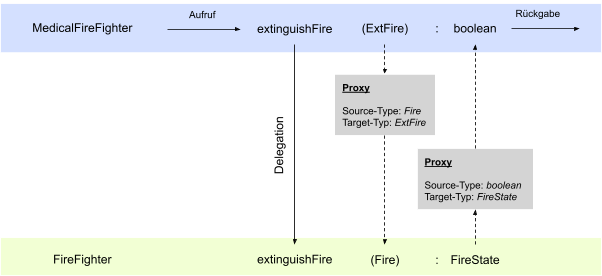
\includegraphics[width=\linewidth]{MDEL_extinguishFire}
\caption{Delegation der Methode $\texttt{extinguishFire}$ mit Typkonvertierungen}
\label{fig:DEL_extinguishFire}
\end{figure}
\noindent
Wie die Proxies generiert werden, wird im folgenden Abschnitt beschrieben.

\subsection{Generierung von Proxies}
Wie im Abschnitt \ref{sec:proxygram} bereits erwähnt, soll die Menge der Proxies für einen Source-Typ $S$ und einer Menge von Target-Typen $T$ über die Funktion $\mathit{proxies(S,T)}$ beschrieben werden.\\\\
In Abhängigkeit von dem Matching zwischen dem Source-Typ und den Target-Typen werden unterschiedliche Arten von Proxies generiert. Für die unterschiedlichen Proxy-Arten gibt es ebenfalls Funktionen, die eine Menge von Proxies zu einem Source-Typen $S$ und einer Menge von Target-Typen $T$ beschreiben.\\\\
In den folgenden Abschnitten werden diese Funktionen für die einzelnen Proxy-Arten beschrieben. Dabei ist davon auszugehen, dass die Proxies eine allgemeine Struktur haben, die in Abschnitt \ref{sec:proxygram} aufgeführt ist. Um die Regeln für die Generierung der Proxies zu beschreiben, soll davon ausgegangen werden, dass jedes Listen-Attribut ($\mathit{NT.}\text{*}$) aus Tabelle \ref{tab:attrGrProxies} ein Attribut $\texttt{len}$ enthält in dem die Anzahl der in der Liste befindlichen Elemente abgelegt ist.


\subsubsection{Sub-Proxy}
Die Voraussetzung für die Erzeugung eines \emph{Sub-Proxies} vom Typ $T$ aus einem Target-Typ $T'$ ist $T \Rightarrow_{spec} T'$. Damit ist der \emph{SpecTypeMatcher} der Basis-Matcher für den Sub-Proxy.
\paragraph{Beispiel}
Als Beispiel soll  der Typ $\texttt{Patient}$ als Source-Typ und der Typ $\texttt{Injured}$ als Target-Typ verwendet werden. Da $\texttt{Patient} \Rightarrow_{spec} \texttt{Injured}$ gilt, kann ein \emph{Sub-Proxy} für diese Konstellation erzeugt werden. Der resultierende \emph{Sub-Proxy} ist im folgenden Listing aufgeführt.
\begin{lstlisting}[style = dsl, caption = Sub-Proxy für Patient, captionpos = b]
proxy for Patient with [Injured]{
	Patient.heal(Medicine):void --> Injured.heal(Medicine):void
	Patient.getName():String --> err
}
\end{lstlisting}
Der abstrakte Syntaxbaum mit den dazugehörigen Attributen ist Abbildung \ref{fig:ASTSUB} zu entnehmen. \footnote{Es wurden nur die Nonterminale mit den dazugehörigen Attributen aufgeführt.}
\begin{figure}[h!]
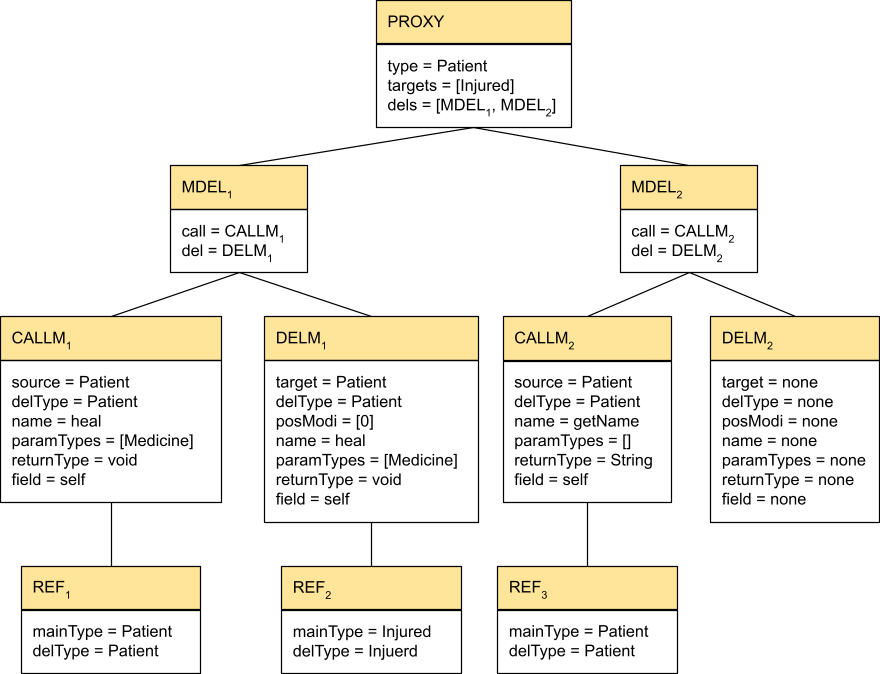
\includegraphics[width=\linewidth]{AST_SubExample}
\caption{AST für das Beispiel zum Sub-Proxy}
\label{fig:ASTSUB}
\end{figure}
\noindent
Der Proxy bietet alle Methoden an, die auch von dessen Source-Typ angeboten werden. Die Methodendelegationen innerhalb des Proxies, beschreiben, was beim Aufruf der jeweiligen aufgerufenen Methoden passiert. So wird ein Aufruf der Methode $\texttt{heal}$ an die Methode $\texttt{heal}$ aus dem Target-Typ delegiert. Ein Aufruf der Methode $\texttt{getName}$ hingegen führt zu einem Fehler, weil keine Delegationsmethode zur Verfügung steht.\\\\
Im Hinblick darauf, dass eine Konvertierung von einem Super-Typ und einen Sub-Typ (Down-Cast) ebenfalls dazu führt, dass bestimmte Methoden, wie in diesem Fall $\texttt{getName}$ nicht ausgeführt werden können, spiegelt der \emph{Sub-Proxy} dieses Verhalten wieder.
\paragraph{Formalisierung}
Formal wird ein \emph{Sub-Proxy} durch die Regeln beschrieben, die im Folgenden vorgestellt werden. Ein \emph{Sub-Proxy} enthält genau einen Target-Typ. Für einen Proxy $P$ wird dieser Sachverhalt durch die folgende Regel dargestellt.
\begin{gather*}
\frac{|\mathit{P.targets}| = 1 \wedge \forall \mathit{T'} \in \mathit{P.targets}: T = T'}{\mathit{targets_{single}(P,T)}}
\end{gather*}
Darüber hinaus enthält ein \emph{Sub-Proxy} $P$ eine bestimmte Menge von Methoden-Delegationen. Dabei muss in allen Methodendelegationen das Attribut $\texttt{field}$ der aufgerufenen Methoden mit dem der Delegationsmethoden übereinstimmen. Folgende Regel stellt diesen Sachverhalt für eine Menge von Methoden-Delegationen $\mathit{MDList}$ dar.
\begin{gather*}
\frac{\splitfrac{\forall \mathit{MD_1}\in \mathit{MDList}: \neg(\exists \mathit{MD_2} \in \mathit{MDList}:\mathit{MD_1.call.field} \neq \mathit{MD_2.call.field}}{ \vee \mathit{MD_1.del.field} \neq \mathit{MD_2.del.field} )}}
{\mathit{equalRefs(MDList)}}
\end{gather*}
Für jede einzelne Methoden-Delegation $\mathit{MD}$ gilt weiterhin, dass die aufgerufene Methode und die Delegationsmethode denselben Namen haben.
\begin{gather*}
\frac{\mathit{MD.call.name} = \mathit{MD.del.name}}
{\mathit{methDel_{nominal}(MD)}}
\end{gather*}
Die aufgerufene Methode muss dabei generell im Typ aus dem Attribut $\texttt{call.delType}$ deklariert sein und die Delegationsmethode im Typ aus dem Attribut $\texttt{del.delType}$.
\begin{gather*}
\frac{\exists \mathit{T'\text{ } m(T)} \in \mathit{methoden(MD.call.delType)}: \mathit{MD.call.name} = m}
{\mathit{callMethod_{simple}(MD)}}
\end{gather*}
\begin{gather*}
\frac{\exists \mathit{T'\text{ }m(T)} \in \mathit{methoden(MD.del.delType)}: \mathit{MD.del.name} = m}
{\mathit{delMethod_{simple}(MD)}}
\end{gather*}
Zusätzlich muss das Attribut $\texttt{field}$ im Attribut $\texttt{call}$ mit dem Wert $\texttt{self}$ belegt und das Attribut $\texttt{mainType}$ mit dem Source-Typ des Proxies belegt sein.
\begin{gather*}
\frac{\mathit{MD.call.mainType} = \mathit{P.type} \wedge \mathit{MD.call.field} = \mathit{self}}
{\mathit{callMethodDelType_{simple}(MD, P)}}
\end{gather*}
Damit ist auch automatisch gewährleistet, dass die Attribute $\texttt{mainType}$ und $\texttt{delType}$ im Attribut $\texttt{call}$ übereinstimmen. (siehe Tabelle \ref{tab:attrGrProxies})\\\\
Ähnliches gilt für die Attribute $\texttt{field}$ und $\texttt{mainType}$ im Attribut $\texttt{del}$. Hierbei muss der Wert des Attributs $\texttt{mainType}$ jedoch mit dem Target-Typ des Proxies übereinstimmen.
\begin{gather*}
\frac{\mathit{MD.del.field} = \mathit{self} \wedge  \mathit{MD.del.mainType} \in \mathit{P.targets} }
{\mathit{delMethodDelType_{simple}(MD, P)}}
\end{gather*}
Damit ist wiederum automatisch gewährleistet, dass die Attribute $\texttt{mainType}$ und $\texttt{delType}$ im Attribut $\texttt{del}$ übereinstimmen. (siehe Tabelle \ref{tab:attrGrProxies})\\\\
Die Regeln für die linke Seite einer Methoden-Delegation $\mathit{MD}$ innerhalb eines \emph{Sub-Proxies} $P$ können damit in folgender Regel zusammengefasst werden:
\begin{gather*}
\frac{\mathit{callMethod_{simple}(MD)} \wedge \mathit{callMethodDelType_{simple}(MD,P)}}
{\mathit{call_{simple}(MD,P)}}
\end{gather*}
Analog dazu können auch die Regeln für die rechte Seite einer Methoden-Delegation $\mathit{MD}$ innerhalb eines \emph{Sub-Proxies} $P$ zusammengefasst werden:
\begin{gather*}
\frac{\mathit{delMethod_{simple}(MD)} \wedge \mathit{delMethodDelType_{simple}(MD,P)}}
{\mathit{del_{simple}(MD,P)}}
\end{gather*}
Im \emph{Sub-Proxy} ist darüber hinaus noch die Methoden-Delegation zu beachten, die bei einem Aufruf zu einem Fehler führt. Dieser Fall wird für eine Methoden-Delegation $\mathit{MD}$ wie folgt beschrieben:
\begin{gather*}
\frac{\mathit{MD.del.name} = \mathit{none}}
{\mathit{del_{err}(MD)}}
\end{gather*}
Die genannten Regeln für eine Methoden-Delegation $\mathit{MD}$ in einem \emph{Sub-Proxy} lassen sich über die beiden folgenden Regeln beschreiben:
\begin{gather*}
\frac{\mathit{call_{simple}(MD,P)} \wedge \mathit{del_{simple}(MD,P) \wedge \mathit{methDel_{nominal}(MD)}}}
{\mathit{methDel_{sub}(MD,P)}}
\end{gather*}
\begin{gather*}
\frac{\mathit{call_{simple}(MD,P)}\wedge\mathit{del_{err}(MD)}
}
{\mathit{methDel_{sub}(MD,P)}}
\end{gather*}
Innerhalb eines \emph{Sub-Proxies} gibt es für jede Methode $m$ des Source-Typ genau eine Methoden-Delegation mit der Methode $m$ als aufgerufene Methode. Damit lässt sich für einen Proxy $P$ in Bezug auf alle seine Methoden-Delegationen folgende Regeln formulieren:
\begin{gather*}
\frac{\splitfrac{\mathit{M} = \mathit{methoden(P.type)}\wedge|\mathit{M}| = |P.dels| \wedge \forall \mathit{T'\text{ }m(T)} \in \mathit{M}:}{\exists \mathit{MD} \in \mathit{P.dels}:m = \mathit{MD.call.name} \wedge \mathit{methDel_{sub}(MD,P)
 }}
}
{\mathit{methDelList_{sub}(P)}}
\end{gather*}
Für einen Proxy $P$ kann die Regel $\mathit{equalRefs(P)}$ im Allgemeinen mit der Bedingung zusammengefasst werden, die besagt, dass ein Proxy immer einen bestimmten Source-Typ $S$ haben muss. Die zusammengefasste Regel lautet:
\begin{gather*}
\frac{\mathit{P.type} = \mathit{S} \wedge \mathit{equalRefs(P)}}{\mathit{proxy(P,S)}}
\end{gather*}
\noindent
Die Menge der \emph{Sub-Proxies}, die mit dem Source-Typ $T$ und dem Target-Typ $T'$ erzeugt werden, wird durch die folgende Funktion beschrieben.
\begin{gather*}
\mathit{proxies_{sub}(T,T')} := 
\left\{\begin{array}{l|l}
		& \mathit{proxy(P,T)}\wedge \mathit{ } \\
	P	& \mathit{targets_{single}(P,T')} \wedge \mathit{ } \\
		& \mathit{methDelList_{sub}(P)}
		 \end{array}
\right\}
\end{gather*}


\subsubsection{Content-Proxy}
Die Voraussetzung für die Erzeugung eines \emph{Content-Proxies} vom Typ $T$ aus einem Target-Typ $T'$ ist $T \Rightarrow_{content} T'$. Damit ist der \emph{ContentTypeMatcher} der Basis-Matcher für den \emph{Content-Proxy}.
\paragraph{Beispiel} Als Beispiel sollen die Typen $\texttt{Medicine}$ und $\texttt{MedCabinet}$ verwendet werden, welche ein Matching der Form $\texttt{Medicine} \Rightarrow_{content} \texttt{MedCabinet}$ aufweisen. Daher kann ein \emph{Content-Proxy} für diese Konstellation erzeugt werden. Ein resultierender \emph{Content-Proxy} ist in folgendem Listing aufgeführt.
\begin{lstlisting}[style = dsl, caption = Content-Proxy für Medicine, captionpos = b]
proxy for Medicine with [MedCabinet]{
	Medicine.getDesciption():String --> MedCabinet.med.getDesciption():String
}
\end{lstlisting}
Durch die Methoden-Delegation dieses \emph{Content-Proxies} wird die Methode $\texttt{getDescription}$ an das Feld $\texttt{med}$ des Target-Typen $\texttt{MedCabniet}$ delegiert.\\\\
Der abstrakte Syntaxbaum mit den dazugehörigen Attributen ist Abbildung \ref{fig:ASTCONTENT} zu entnehmen. \footnote{Es wurden nur die Nonterminale mit den dazugehörigen Attributen aufgeführt.}
\begin{figure}[h!]
\centering
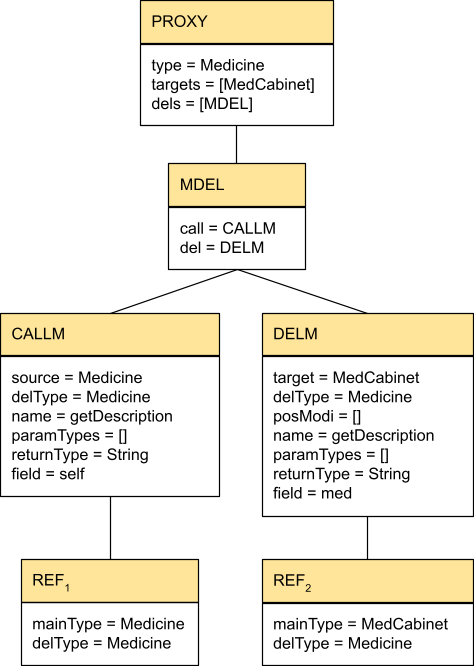
\includegraphics[width=0.5\linewidth]{AST_ContentExample}
\caption{AST für das Beispiel zum Content-Proxy}
\label{fig:ASTCONTENT}
\end{figure}
\noindent
\paragraph{Formalisierung}
Formal wird ein \emph{Content-Proxy} durch die Regeln beschrieben, die im Folgenden vorgestellt werden.\\\\
Ein \emph{Content-Proxy} enthält, wie auch der \emph{Sub-Proxy}, genau einen Target-Typ. Ebenfalls identisch zum \emph{Sub-Proxy} sind die Bedingungen hinsichtlich der aufgerufenen Methoden in den einzelnen Methoden-Delegationen.\\\\
In den Delegationsmethoden einer einzelnen Methoden-Delegation $\mathit{MD}$ dürfen die Attribute $\texttt{mainType}$ und $\texttt{delType}$ im \emph{Content-Proxy} nicht identisch sein. Dementsprechend darf das Attribut $\texttt{field}$ nicht mit dem Wert $\texttt{self}$ belegt sein. Vielmehr muss für das Attribut $\texttt{delTyp}$ und den Source-Typ $T$ des Proxies ein Matching der Form $T \Rightarrow_{internCont} \mathit{MD.del.delTyp}$ gelten. Daher gilt für den \emph{Content-Proxy} die folgende Regel:
\begin{gather*}
\frac{\mathit{P.type} \Rightarrow_{internCont} \mathit{MD.del.delType}  \wedge \mathit{MD.del.mainType} \in \mathit{P.targets}}
{\mathit{delMethodDelType_{content}(MD,P)}}
\end{gather*}
\noindent
Damit kann eine zusammenfassende Regel für die Delegationsmethoden einer Methoden-Delegation $\mathit{MD}$ wie folgt definiert werden:
\begin{gather*}
\frac{\mathit{delMethod_{simple}(MD)} \wedge \mathit{delMethodDelType_{content}(MD,P)}}
{\mathit{del_{content}(MD,P)}}
\end{gather*}
Die zusammenfassende Regel für eine einzelne Methoden-Delegation $\mathit{MD}$ innerhalb eines \emph{Content-Proxies} hat die folgende Form:
\begin{gather*}
\frac{\mathit{call_{simple}(MD,P)} \wedge \mathit{del_{content}(MD,P) \wedge \mathit{methDel_{nominal}(MD)}}}
{\mathit{methDel_{content}(MD,P)}}
\end{gather*}
Wie auch im \emph{Sub-Proxy} gibt es im \emph{Content-Proxy} für jede Methode $m$ des Source-Typen genau eine Methoden-Delegation mit der Methode $m$ als aufgerufene Methode. Daraus ergibt sich für alle Methoden-Delegationen aus einem \emph{Content-Proxy} $P$ folgende Regel:
\begin{gather*}
\frac{\splitfrac{M = \mathit{methoden(P.type) }\wedge|\mathit{M}| = |\mathit{P.dels}| \wedge \forall \mathit{T' \text{ }m(T)} \in \mathit{M}:}{ \exists \mathit{MD} \in \mathit{P.dels}:m = \mathit{MD.call.name} \wedge \mathit{methDel_{content}(MD,P)
 }
}}
{methDelList_{content}(P)}
\end{gather*}
Die Menge der \emph{Content-Proxies}, die mit dem Source-Typ $T$ und dem Target-Typ $T'$ erzeugt werden, wird durch die folgende Funktion beschrieben.
\begin{gather*}
\mathit{proxies_{content}(T,T')} := 
\left\{\begin{array}{l|l}
		& \mathit{proxy(P,T)} \wedge \mathit{ } \\
	P	& \mathit{targets_{single}(P,T')} \wedge \mathit{ }\\
		& \mathit{methDelList_{content}(P)} 
		 \end{array}
\right\}
\end{gather*}
\subsubsection{Container-Proxy}
Die Voraussetzung für die Erzeugung eines \emph{Container-Proxies} vom Typ $T$ aus einem Target-Typ $T'$ ist $T \Rightarrow_{container} T'$. Damit ist der \emph{ContainerTypeMatcher} der Basis-Matcher für den \emph{Container-Proxy}.
\paragraph{Beispiel}
Als Beispiel werden wiederum die Typen $\texttt{Medicine}$ und $\texttt{MedCabinet}$ verwendet, welche ein Matching der Form $\texttt{MedCabinet} \Rightarrow_{container} \texttt{Medicine}$ aufweisen. Daher kann ein \emph{Content-Proxy} für diese Konstellation erzeugt werden. Ein resultierender \emph{Content-Proxy} ist in folgendem Listing aufgeführt.
\begin{lstlisting}[style = dsl, caption = Container-Proxy für MedCabniet, captionpos = b ]
proxy for MedCabinet with [Medicine]{
	MedCabinet.med.getDesciption():String --> Medicine.getDesciption():String
}
\end{lstlisting}
Durch die Methoden-Delegation dieses \emph{Container-Proxies} findet eine Delegation nur dann statt, wenn die Methoden $\texttt{getDescription}$ auf dem Feld $\texttt{med}$ des Source-Typ aufgerufen wird. Diese wird dann an den Target-Typen $\texttt{MedCabniet}$ delegiert.\\\\
Der abstrakte Syntaxbaum mit den dazugehörigen Attributen ist Abbildung \ref{fig:ASTCONTAINER} zu entnehmen. \footnote{Es wurden nur die Nonterminale mit den dazugehörigen Attributen aufgeführt.}
\begin{figure}[h!]
\centering
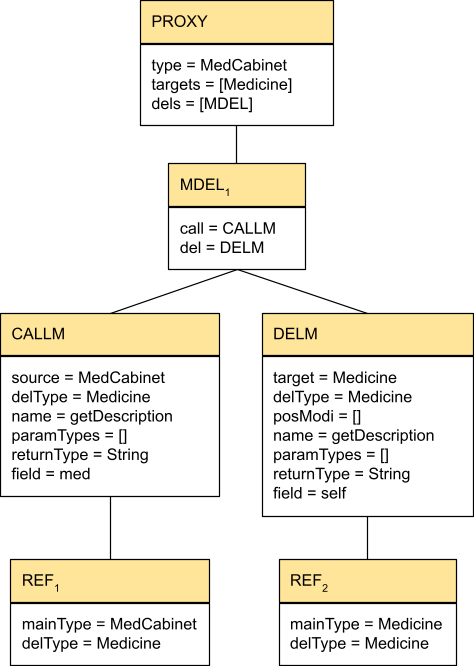
\includegraphics[width=0.5\linewidth]{AST_ContainerExample}
\caption{AST für das Beispiel zum Container-Proxy}
\label{fig:ASTCONTAINER}
\end{figure}
\noindent
\paragraph{Formalisierung}
Formal wird ein \emph{Container-Proxy} durch die Regeln beschrieben, die im Folgenden vorgestellt werden.\\\\
Ein \emph{Container-Proxy} enthält, wie die vorher beschriebenen Proxies, genau einen Target-Typ. Die Eigenschaften der Delegationsmethoden innerhalb der einzelnen Methoden-Delegationen gleichen denen aus dem \emph{Sub-Proxy}.\\\\
In den angerufenen Methoden einer einzelnen Methoden-Delegation $\mathit{MD}$ dürfen die Attribute $\texttt{mainType}$ und $\texttt{delType}$ im \emph{Container-Proxy} nicht übereinstimmen. Dementsprechend darf das Attribut $\texttt{field}$ nicht mit dem Wert $\texttt{self}$ belegt sein. Vielmehr müssen der Wert des Attributs $\texttt{delTyp}$ und der Target-Typ $T$ des Proxies ein Matching der Form $T \Rightarrow_{internCont} \texttt{delTyp}$ ausweisen. Daher gilt für den \emph{Container-Proxy} $P$ folgende Regel.
\begin{gather*}
\frac{\splitfrac{\mathit{MD.call.mainType} = \mathit{P.type} \wedge \forall \mathit{T} \in \mathit{P.targets}:}
{  \mathit{T} \Rightarrow_{internCont} \mathit{MD.call.delType}}
}
{\mathit{callMethodDelType_{container}(MD,P)}}
\end{gather*}
\noindent
Damit kann eine zusammenfassende Regel für die aufgerufenen Methoden wie folgt definiert werden:
\begin{gather*}
\frac{\mathit{callMethod_{simple}(MD)} \wedge \mathit{callMethodDelType_{container}(MD,P)}}
{\mathit{call_{container}(MD,P)}}
\end{gather*}
Die zusammenfassende Regel für eine einzelne Methoden-Delegation $\mathit{MD}$ innerhalb eines \emph{Container-Proxies} hat die folgende Form:
\begin{gather*}
\frac{\mathit{call_{container}(MD,P)} \wedge \mathit{del_{simple}(MD,P)} \wedge \mathit{methDel_{nominal}(MD)}}
{\mathit{methDel_{container}(MD,P)}}
\end{gather*}
Für einen \emph{Container-Proxy} $P$ gilt ebenfalls die Regel $\mathit{equalRefs(P.dels)}$. Daher müssen die Werte des Attributs $\texttt{call.delType}$ aller Methoden-Delegationen des Proxies $P$ übereinstimmen. Ferner muss es für jede Methode $m$ des Typen aus $\texttt{call.delType}$ genau eine Methoden-Delegation mit der Methode $m$ als aufgerufene Methode existieren. Daraus ergibt sich für alle Methoden-Delegationen aus einem \emph{Content-Proxy} $P$ folgende Regel:
\begin{gather*}
\frac{\splitfrac{\mathit{M} = \mathit{methoden(P.dels[0].call.delType)} \wedge |\mathit{M}| = |P.dels| \wedge \forall \mathit{T' \text{ } m(T)} \in \mathit{M}:}
{\exists \mathit{MD} \in P.dels:m = \mathit{MD.call.name} \wedge \mathit{methDel_{container}(MD,P)}
 }}
{\mathit{methDelList_{container}(P)}}
\end{gather*}
Die Menge der \emph{Container-Proxies}, die mit dem Source-Typ $T$ und dem Target-Typ $T'$ erzeugt werden, wird durch die folgende Funktion beschrieben.
\begin{gather*}
\mathit{proxies_{container}(T,T')} := 
\left\{\begin{array}{l|l}
		& \mathit{proxy(P,T)}  \wedge \mathit{ } \\
	P	& \mathit{target_{single}(P,T')} \wedge \mathit{ } \\
		& \mathit{methDelList_{container}(P)} 
		 \end{array}
\right\}
\end{gather*}

\subsubsection{Struktureller Proxy}
Die Voraussetzung für die Erzeugung eines \emph{strukturellen Proxies} vom \emph{required Typ} $R$ aus einem Target-Typ $T$ ist $R \Rightarrow_{struct} T$. Damit ist der \emph{StructuralTypeMatcher} der Basis-Matcher für den \emph{strukturellen Proxy}.\\\\
Der \emph{strukturelle Proxy} ist der einzige Proxy, der mit mehreren Target-Typen erzeugt werden kann. 
\paragraph{Beispiel}
Als Beispiel werden die Typen $\texttt{MedicalFireFighter}$, $\texttt{Doctor}$ und $\texttt{FireFighter}$ verwendet. Dabei ist $\texttt{MedicalFireFighter}$ der Source-Typ des Proxies und die Menge der anderen beiden Typen bilden die Target-Typen des Proxies. Da der Source-Typ zu den Target-Typen ein Matching der Form $\texttt{MedicalFireFighter} \Rightarrow_{struct} \texttt{FireFighter}$ bzw. $\texttt{MedicalFireFighter} \Rightarrow_{struct} \texttt{Doctor}$ aufweist, kann ein \emph{struktureller Proxy} erzeugt werden. Ein solcher ist in folgendem Listing aufgeführt.
\begin{lstlisting}[style = dsl, caption = Struktureller Proxy für MedicalFireFighter, captionpos = b]
proxy for MedicalFireFighter with [Doctor, FireFighter]{
	MedicalFireFighter.heal(Patient, MedCabinet):void --> Doctor.heal(Patient, Medicine):void
	MedicalFireFighter.extinguishFire(ExtFire):boolean --> FireFighter.extinguishFire(Fire):FireState
}
\end{lstlisting}
In diesem Beispiel wird der Methodenaufruf der Methode $\texttt{heal}$ auf dem Proxy an die Methode $heal$ des Typs $\texttt{Doctor}$ delegiert. Analog dazu würde ein Aufruf der Methode $\texttt{extinguishFire}$ auf dem Proxy an die Methode $extinguishFire$ des Typs $\texttt{FireFighter}$ delegiert werden. Die Methoden stimmen jeweils strukturell überein.\\\\
Der abstrakte Syntaxbaum mit den dazugehörigen Attributen ist Abbildung \ref{fig:ASTSTRUCT} zu entnehmen. \footnote{Es wurden nur die Nonterminale mit den dazugehörigen Attributen aufgeführt.}
\begin{figure}[h!]
\centering
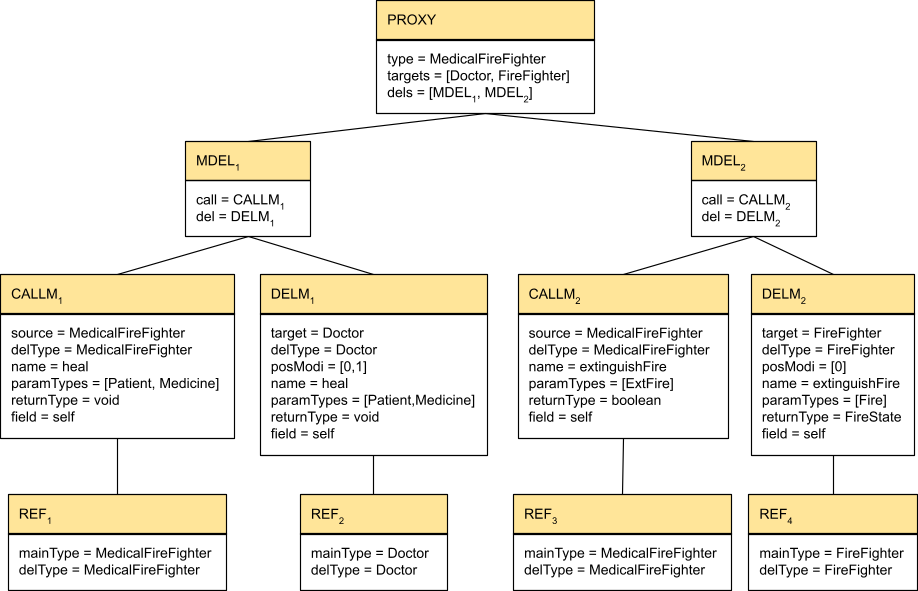
\includegraphics[width=\linewidth]{AST_StructExample}
\caption{AST für das Beispiel zum strukturellen Proxy}
\label{fig:ASTSTRUCT}
\end{figure}
\noindent
\paragraph{Formalisierung}
Ein \emph{struktureller Proxy} wird formal durch die folgenden Regeln beschrieben.\\\\
Ein \emph{struktureller Proxy} kann, wie bereits erwähnt, mehrere Target-Typen enthalten.
Für jeden Target-Typ $T$ muss dabei jedoch wenigstens eine Delegationsmethode im Proxy mit einem Attribut $\texttt{target} = T$ existiert. Dadurch gilt die für einen \emph{strukturellen Proxy} Proxy $P$:
\begin{gather*}
\frac{\forall \mathit{T} \in \mathit{P.targets}:\exists \mathit{MD} \in \mathtt{P.dels}:\mathit{MD.del.target} = T}{\mathit{targets_{struct}(P, T)}}
\end{gather*}
Für die aufgerufene Methode und die Delegationsmethode einer einzelnen Methoden-Delegation $\mathit{M}$ gelten im \emph{strukturellen Proxy} dieselben Regeln wie für den \emph{Sub-Proxy}. Die Namen der aufgerufenen Methode und der Delegationsmethode müssen dabei jedoch nicht übereinstimmen. Dafür müssen diese beiden Methode jedoch ein strukturelles Matching aufweisen. Bezogen auf die Rückgabe-Typen einer aufgerufenen Methode $\mathit{C}$ und der Delegationsmethode $\mathit{D}$ aus einer Methoden-Delegation muss daher Folgendes gelten.
\begin{gather*}
\frac{\mathit{D.returnType} \Rightarrow_{internStruct} \mathit{C.returnType}}{\mathit{return_{struct}(C,D)}}
\end{gather*} 
Weiterhin muss für die Parameter-Typen gelten:
\begin{gather*}
\frac{\mathit{C.paramCount} = 0}{\mathit{params_{struct}(C,D)}}
\end{gather*} 
\begin{gather*}
\frac{\splitfrac{\forall \mathit{i} \in \{0,...,\mathit{C.paramCount}-1\}:}
{ \mathit{C.paramTypes}[i] \Rightarrow_{internStruct} \mathit{D.paramTypes}[\mathit{D.posModi}[i]]
}}{\mathit{params_{struct}(C,D)}}
\end{gather*} 
Für eine einzelne Methoden-Delegation $\mathit{MD}$ eines \emph{strukturellen Proxies} $P$ kann dann folgende Regel aufgestellt werden.
\begin{gather*}
\frac{\splitfrac{\mathit{call_{simple}(MD,P)} \wedge \mathit{del_{simple}(MD,P)} \wedge} {\mathit{return_{struct}(MD.call, MD.del)} \wedge \mathit{params_{struct}(MD.call, MD.del)}}
}
{\mathit{methDel_{struct}(MD,P)}}
\end{gather*}
In einem \emph{strukturellen Proxy} muss für jede Methode $m$ des Source-Typen genau eine Methoden-Delegation mit der Methode $m$ als aufgerufene Methode existieren. Daraus ergibt sich für alle Methoden-Delegationen aus einem \emph{strukturellen Proxy} $P$ folgende Regel:
\begin{gather*}
\frac{\splitfrac{\mathit{M} = \mathit{methoden(P.type)} \wedge |\mathit{M}| = |\mathit{P.dels}| \wedge \forall \mathit{T' \text{ }m(T)} \in \mathit{M}:}{\exists \mathit{MD} \in \mathit{P.dels}:\mathit{MD.call.name} = m \wedge \mathit{methDel_{struct}(MD,P)}
 }
}
{\mathit{methDelList_{struct}(P)}}
\end{gather*}
Wie in Abschnitt 
Die Menge der \emph{strukturellen Proxies}, die mit dem Source-Typ $R$ und der Menge von Target-Typen $T$ erzeugt werden, wird durch die folgende Funktion beschrieben.
\begin{gather*}
\mathit{proxies_{struct}(R,T)} := 
\left\{\begin{array}{l|l}
		& \mathit{proxy(P,R)}\wedge \mathit{ }\\
	P	& \mathit{targets_{struct}(P,T)} \wedge \mathit{ }\\
		& \mathit{methDelList_{struct}(P)}  
		 \end{array}
\right\}
\end{gather*}

\paragraph{Allgemeine Generierung von Proxies}
Die Proxy-Funktion der einzelnen Proxy-Arten werden zur Beschreibung einer allgemeine Funktion für die Generierung der Proxies verwendet. Dazu sind die Proxy-Arten zusammen mit den dazugehörigen Matchingrelationen und Proxy-Fukntionen in Tabelle \ref{tab:baseMatcher} noch einmal aufgeführt.

\begin{table}[H]
\centering
\begin{tabular}{|c|c|c|}
\hline
\hline
\centering\textbf{Proxy-Art} & \textbf{Matchingrelation} & \textbf{Funktionsname}\\
\hline
\hline
Sub-Proxy
&  
$\Rightarrow_{spec}$
& 
$\mathit{proxies_{sub}}$
\\
\hline
Content-Proxy
& 
$\Rightarrow_{content}$
& 
$\mathit{proxies_{content}}$
\\
\hline
Container-Proxy
& 
$\Rightarrow_{container}$
& 
$\mathit{proxies_{container}}$
\\
\hline
struktureller Proxy
&
$\Rightarrow_{struct}$
& 
$\mathit{proxies_{struct}}$
 \\
\hline
\hline
\end{tabular}
\caption{Proxy-Arten mit Matchingrelationen und Proxy-Funktionen}
 \label{tab:baseMatcher}
\end{table}
\noindent
Die im Abschnitt \ref{sec:proxygram} erwähnte Funktion $\mathit{proxies(S,T)}$ kann darauf aufbauend für einen Source-Typ $S$ und eine Menge von Target-Typen $T$ wie folgt beschrieben werden.
\begin{gather*}
\mathit{proxies(S,T)} := 
\left\{\begin{array}{ll}
\mathit{proxy_{sub}(S,T)}	& \text{wenn } |T| = 1 \wedge \mathit{ }\\
& \forall T' \in T: S \Rightarrow_{sub} T'\\	
&\\
\mathit{proxy_{content}(S,T)}	& \text{wenn } |T| = 1 \wedge \mathit{ }\\
& \forall T' \in T: S \Rightarrow_{content} T' \\
&\\
\mathit{proxy_{container}(S,T)} & \text{wenn } |T| = 1 \wedge \mathit{ } \\
& \forall T' \in T: S \Rightarrow_{container} T' \\
&\\
\mathit{proxy_{struct}(S,T)} & \text{wenn } |T| > 0 \wedge \mathit{ } \\
&\forall T' \in T: S \Rightarrow_{struct} T'
		 \end{array}
\right\}
\end{gather*}
\subsection{Anzahl möglicher Proxies innerhalb einer Bibliothek}
Die Generierung der Proxies für ein required Typ $R$ aus der Bibliothek $L$ erfolgt während der Exploration mit den Mengen von provided Typen aus $\mathit{cover(R,L)}$ (siehe Abschnitt \ref{sec_ergStructEval}). Mit einer Menge $T \in \mathit{cover(R,L)}$ können durchaus mehrere Proxies erzeugt werden. Das ist dann der Fall, wenn mehrere der Methoden, die in den provided Typen aus $T$ deklariert wurden, mit einer Methode des required Typs $R$ strukturell übereinstimmen.
Die Anzahl der möglichen Proxies für ein required Typ $R$ mit einer bestimmten Mengen von Target-Typen $T_1,...,T_k$ ist somit von der Anzahl der Methoden abhängig, die in einem der Target-Typen des Proxies deklariert wurden und strukturell mit den Methoden aus $R$ übereinstimmen. 
\\\\
Die Menge der Methoden eines provided Typen $P$, die strukturell mit einer Methode $m$ übereinstimmen, wird über die Funktion $\mathit{structM_{target}}$ beschrieben.
\begin{gather*}
\mathit{structM_{target}(m, P)} := 
\left\{\begin{array}{l|l}
m'	& m' \in \mathit{methoden(P)} \wedge  m \Rightarrow_{method} m'
\end{array}
\right\}
\end{gather*}
\noindent
Darauf aufbauend wird die Menge der Methoden einer Menge von \emph{provided Typen} $T$, die strukturell mit einer Methode $m$ übereinstimmen, über die Funktion $\mathit{structM_{targetset}}$ beschrieben.
\begin{gather*}
\mathit{structM_{targetset}(m, T)} := 
\left\{\begin{array}{l|l}
m'	& \exists P \in T: m' \in \mathit{structM_{target}(m,P)}
\end{array}
\right\}
\end{gather*}
\noindent
Sei $R$ ein \emph{required Typ} und $T$ eine Menge von \emph{provided Typen} innerhalb einer Bibliothek $L$ mit $T \in \mathit{cover(R,L)}$. Dann bildet die Funktion $\mathit{structMSets}$ die Mengen der Methoden aus den \emph{provided Typen} ab, die mit jeweils einer Methode aus $R$ gematcht werden können.
\begin{gather*}
\mathit{structMSets(R,T)} := 
\left\{M
\begin{array}{l|l}
&\exists \mathit{m} \in \mathit{methoden(R)} : 
\\
&M = \mathit{structM_{targetset}(m,T)}
\end{array}
\right\}
\end{gather*}
\noindent
%Dann bilden $M_1,...,M_n$ wie folgt die Mengen der Methoden der Target-Typen in $T$, die mit jeweils einer Methode $m_i \in \mathit{methoden(R)}$  strukturell übereinstimmen.
%\begin{gather*}
%M_1 = \mathit{structM_{target}(m_1,T)}\\
%...\\
%M_n = \mathit{structM_{target}(m_n,T)}
%\end{gather*}
Für jede Kombination von jeweils einem Element aus jeder der Mengen aus $\mathit{structMSets(R,T)}$ kann ein Proxy für $R$ mit der Menge der Target-Typen $T$ erzeugt werden.

\begin{example}{bsp_structmtarget}
Aufbauend auf dem vorherigen Beispiel \ref{bsp_cover} ergeben sich für die Menge der Target-Typen  $\{\texttt{Leave}, \texttt{Come}\}$ und die beiden Methoden des required Typs $\texttt{Greeting}$ folgende Menge von übereinstimmenden Methoden über die Funktion $\mathit{structMSets}$:
\begin{gather*}
\mathit{structMSets(\methodForm{String}{hello}{},\{\texttt{Leave}, \texttt{Come}\})} = 
\left\{
\begin{array}{l}
\methodForm{String}{hello}{},\\
\methodForm{String}{goodMorning}{},\\
\methodForm{String}{bye}{}
\end{array}
\right\}\\
\mathit{structMSets(\methodForm{String}{bye}{},\{\texttt{Leave}, \texttt{Come}\})} = 
\left\{
\begin{array}{l}
\methodForm{String}{hello}{},\\
\methodForm{String}{goodMorning}{},\\
\methodForm{String}{bye}{}
\end{array}
\right\}
\end{gather*}
\noindent
Darauf aufbauend lassen sich die folgenden vier Proxies mit den Target-Typen $\texttt{Leave}$ und $\texttt{Come}$ erzeugen.
\begin{lstlisting}[style = dsl]
proxy Greeting with [Come, Leave]{
	Greeting.hello():String --> Come.hello():String
	Greeting.bye():String --> Leave.bye():String
}
\end{lstlisting}
\begin{lstlisting}[style = dsl]
proxy Greeting with [Come, Leave]{
	Greeting.hello():String --> Come.goodMorning():String
	Greeting.bye():String --> Leave.bye():String
}
\end{lstlisting}
\begin{lstlisting}[style = dsl]
proxy Greeting with [Come, Leave]{
	Greeting.hello():String --> Leave.bye():String
	Greeting.bye():String --> Come.hello():String
}
\end{lstlisting}
\begin{lstlisting}[style = dsl]
proxy Greeting with [Come, Leave]{
	Greeting.hello():String --> Leave.bye():String
	Greeting.bye():String --> Come.goodMorning():String
}
\end{lstlisting}
\end{example}
\noindent
Für die Bildung eines Proxies wird aus jeder der oben genannten Menge $\{M_1,...,M_n\} = structMSets(R,T)$ genau ein Element als Delegationsmethode verwendet werden. Die Anzahl aller möglichen Proxies für ein \emph{required Typ} $R$ aus einer Menge von Target-Typen $T$ sei über die Funktion $\mathit{proxyCount(R,T)}$ ausgedrückt. Für $\mathit{proxyCount(R,T)}$ ist zu beachten, dass es sich dabei lediglich um eine Annäherung an die tatsächliche Anzahl der Proxies handelt, die unter den oben beschriebenen Bedingungen erzeugt werden können. Dies liegt daran, dass eine Delegationsmethoden $dm \in M_1 \cup ... \cup M_n$ innerhalb eines Proxy maximal einmal verwendet werden darf. Es ist jedoch möglich, dass es zwischen den oben genannten Mengen 
$M_1,...,M_n$ Überschneidungen gibt (siehe vorheriges Beispiel). Daher gelten für die Funktion $\mathit{proxyCount}$ folgende Regeln unter den oben genannten Modalitäten:
\begin{gather*}
\frac{M_1 \cap ... \cap M_n = \emptyset}{\mathit{proxyCount(R,T)} = \prod\limits_{i=1}^{n}|M_i| }
\\\\
\frac{M_1 \cap ... \cap M_n \neq \emptyset}{\mathit{proxyCount(R,T)} < \prod\limits_{i=1}^{n}|M_i| }
\end{gather*}
\noindent
Im Allgemeinen gilt demnach:
\begin{gather*}
\mathit{proxyCount(R,T)} \leq 
\begin{array}{l|l}
\prod\limits_{i=1}^{n}|\mathit{structM_{targetset}(m_i, T)}|
&
\left\{
\begin{array}{l}
m_1,\\
...,\\
m_n
\end{array}
\right\}
= \mathit{methoden(R)}
\end{array}
\end{gather*}
Da innerhalb einer Bibliothek $L$ mehrere Mengen von Target-Typen zur Bildung eines Proxies für einen required Typ $R$ infrage kommen (siehe Funktion $\mathit{cover}$) muss die Anzahl der Proxies über die Funktion $\mathit{proxyCount}$ für alle Elemente aus $\mathit{cover(R,L)}$ ermittelt und summiert werden. Die folgende Funktion beschreibt diesen Sachverhalt für einen required Typ $R$ aus einer Bibliothek $L$.
\begin{gather*}
\mathit{libProxyCount(R,L)} = 
\begin{array}{l|l}
\sum_{i=1}^{n}\mathit{proxyCount(R,c_i)}
&
\left\{
\begin{array}{l}
c_1,\\
...,\\
c_n
\end{array}
\right\} = \mathit{cover(R,L)}
\end{array}
\end{gather*}
\section{Semantische Evaluation}
Das Ziel der semantischen Evaluation ist es, einen der Proxies, die im Rahmen der 1. Stufe der Exploration erzeugt wurden, hinsichtlich der vordefinierten Testfälle zu evaluieren. Da die gesamte Exploration zur Laufzeit des Programms durchgeführt wird, stellt sie hinsichtlich der nicht-funktionalen Anforderungen eine zeitkritische Komponente dar.
\\\\
Da die Anforderungen an die gesuchte Komponente mit bedacht spezifiziert werden müssen, ist es irrelevant, ob es mehrere Proxies gibt, die den vordefinierten Testfällen standhalten. Vielmehr soll bei der semantischen Evaluation lediglich ein Proxy gefunden werden, dessen Semantik zu positiven Ergebnissen hinsichtlich aller vordefinierten Testfälle führt. Somit wird die semantische Evaluation beendet, sobald ein solcher Proxy gefunden ist.
\subsection{Besonderheiten der Testfälle}
Bei den vordefinierten Tests handelt es sich auf formaler Ebene um Typen, die eine eval-Methode mit der Struktur $\texttt{boolean eval( proxy )}$ anbieten, welche einen Proxy als Parameter erwartet und ein Objekt vom Typ $\texttt{boolean}$ zurückgibt. Weiterhin verfügt ein Test über ein Attribut $\texttt{triedMethodCalls}$, in dem eine Liste von Methodennamen des Proxies, die bei der Durchführung der eval-Methode aufgerufen wurden, hinterlegt ist.
\\\\
Die Implementierung der eval-Methode ist an folgende Bedingungen geknüpft:
\begin{enumerate}
\item Vor dem Aufruf einer Methode auf dem als Parameter übergebenen Proxy-Objekt, wird der Name der dieser Methode in der Liste im Feld $\texttt{triedMethodCalls}$ ergänzt.
%\item Nach einem fehlgeschlagenen Aufruf einer Methode auf dem als Parameter übergebenen Proxy-Objekt, wird das Feld $\texttt{failedMethod}$ mit dem Namen der fehlgeschlagenen Methode belegt. Zusätzlich wird die eval-Methode direkt danach mit dem Rückgabewert $\texttt{false}$ beendet.
\item Wenn der Proxy den Test erfüllt, wird der Wert $\texttt{true}$ zurückgegeben. Anderenfalls wird der Wert $\texttt{false}$ zurückgegeben.
\end{enumerate}

\begin{example}{xmpl_evalMethode}
In folgendem Listing \ref{lst_examEval} ist eine eval-Methode aufgeführt, die die oben genannten Bedingungen erfüllt. Es sei davon auszugehen, dass der als Parameter übergebene Proxy eine Methode mit der Struktur $\methodForm{Integer}{add}{Integer x, Integer y}$
anbietet. Der Fehlschlag ($\texttt{err}$) dieser Methode wird über einen Try-Catch-Block abgefangen.
\begin{lstlisting}[style = pseudo, label = lst_examEval, caption = Beispielhafte Implementierung einer eval-Methode, captionpos = b]
function eval( proxy ){
	res = 0	
	triedMethodCalls.add( "add" )
	res = proxy.add(1, 1)
	return res == 2;
}
\end{lstlisting}
\end{example}

\subsection{Algorithmus für die semantische Evaluation}\label{sec_semEvalAlgo}
Bei der Exploration soll letztendlich in einer Bibliothek $L$ zu einem vorgegebenen required Type $R$ ein Proxy gefunden werden. Die Mengen der Target-Typen auf deren Basis mehrere Proxies erzeugt werden können, wurden im Abschnitt \ref{sec_anzahlProxies} über $\mathit{cover(R,L)}$ beschrieben. Die in $T = \mathit{cover(R,L)}$ befindlichen Mengen können eine unterschiedliche Anzahl von Target-Typen enthalten. Die maximale Mächtigkeit einer Menge $T_i \in T$ ist gleich der Anzahl der Methoden in $R$.
\begin{gather*}
\mathit{maxTargets(R)} := |\mathit{methoden(R)}|
\end{gather*}
\noindent
In Bezug zur Funktion $\mathit{cover}$ gilt:
\begin{gather*}
\forall T \in \mathit{cover(R,L)} : |T| \leq \mathit{maxTargets(R)}
\end{gather*}
\noindent
\\
Das in dieser Arbeit beschriebene Konzept basiert auf der Annahme, dass der gesamte Anwendungsfall - oder Teile davon - , der mit der vordefinierten Struktur und den vordefinierten Tests abgebildet werden soll, schon einmal genauso oder so ähnlich in dem gesamten System implementiert wurde. Aus diesem Grund kann für die semantische Evaluation davon ausgegangen werden, dass die erfolgreiche Durchführung aller relevanten Tests umso wahrscheinlicher ist, je weniger Target-Typen im Proxy verwendet werden.
\\\\
Sei folgende Funktion für eine Menge von Target-Typen $T \in \mathit{cover(R,L)}$ und eine ganze Zahl $a > 0$ definiert:
\begin{gather*}
\mathit{targetSets(T,a)} := \{T_i | T_i \in T \wedge |T_i| = a\}
\end{gather*}
\noindent
Ausgehend von einer Bibliothek $L$ kann der Algorithmus für die semantische Evaluation der Proxies, die für einen required Typ $R$ mit den Mengen der Target-Typen $T = \mathit{cover(R, L)}$ erzeugt werden können, und der Menge von Tests (Parameter $\texttt{tests}$) wie folgt im Pseudo-Code beschrieben werden. Die globale Variable $\texttt{passedTests}$ enthält dabei die Anzahl der für den aktuell zu überprüfenden Proxy erfolgreich durchgeführten Tests. Außerdem sei davon auszugehen, dass die Funktionen aus Abschnitt \ref{sec_structEval} wie beschrieben definiert sind.
\begin{lstlisting}[style = pseudo, caption = Semantische Evaluation ohne Heuristiken, captionpos = b, label = lst_semEval]
passedTests = 0

function semanticEval( R, T, tests ){
	for( i = 1; i <= $\mathit{maxTargets( R )}$; i++ ){
		relProxies = relevantProxies( R, T, i )
		proxy = evalProxies( relProxies, tests )	
		if( proxy != null ){
			// passenden Proxy gefunden
			return proxy
		}
	}
	// kein passenden Proxy gefunden
	return null;
}

function relevantProxies(R, T, anzahl){
	proxies = []
	targetSets = $\mathit{targetSets( T, anzahl )}$
	for( targets : targetSets ){
		proxies.addAll( $\mathit{proxies( R, targets )}$ )
	}
	return proxies;
}

function evalProxies(proxies, tests){
	for( proxy : proxies ){
		passedTests = 0
		evalProxy(proxy, tests)
		if( passedTests == tests.size ){
			// passenden Proxy gefunden
			return proxy
		}
	}
	// kein passenden Proxy gefunden
	return null
}

function evalProxy(proxy, tests){
	for( test : tests ){
		if( !test.eval( proxy ) ){
			\\ wenn ein Test fehlschlaegt, dann entspricht der 
			\\ Proxy nicht den semantischen Anforderungen
			return
		}
		passedTests = passedTests + 1
	}
}
\end{lstlisting}
Die Dauer der Laufzeit der in Listing \ref{lst_semEval} definierten Funktionen hängt maßgeblich von der Anzahl der Proxies ab, die für den required Typ $R$ in der Bibliothek $L$ erzeugt werden können (siehe auch Abschnitt \ref{sec_anzahlProxies} Funktion $\mathit{proxyCount}$). Im schlimmsten Fall müssen alle Proxies hinsichtlich der vordefinierten Tests erzeugt und evaluiert werden. Um die Anzahl dieser Proxies zu reduzieren, werden die im folgenden Abschnitt beschriebenen Heuristiken verwendet.


\section{Heuristiken}
Die Heuristiken werden an unterschiedlichen Stellen des Algorithmus aus Listing \ref{lst_semEval} eingebaut. Teilweise ist es für die Verwendung einer Heuristik notwendig, weitere Information während der semantischen Evaluation zu ermitteln und diese zu speichern. In den folgenden Abschnitten werden die Heuristiken und die dafür notwendigen Anpassungen an den jeweiligen Funktionen beschrieben.

%\subsection{Heuristiken für die Optimierung der Reihenfolge}
Die folgenden Heuristiken haben zum Ziel, die Reihenfolge, in der die Proxies hinsichtlich der vordefinierten Tests geprüft werden, so anzupassen, dass ein passender Proxy möglichst früh geprüft wird.


\subsection{Beachtung des Matcherratings (LMF)}\label{sec_lmf}
Bei dieser Heuristik, welche den Namen\emph{low matcherrating first} (kurz: LMF) trägt, werden die Proxies auf der Basis eines so genannten Matcherratings bewertet. Bei dem Matcherrating eines Proxies handelt es sich um einen numerischen Wert. Um diesen Wert zu ermitteln, wird für jede Matchingrelation bzw. für jeden Matcher aus Abschnitt \ref{sec_matcher} ein Basisrating vergeben. Folgende Funktion beschreibt das Basisrating für das Matching zweier Typen $S$ und $T$:
\begin{gather*}
\mathit{base(S,T)} :=  \left\{ 
				\begin{array}{l}
					100 | S \Rightarrow_{exact}  T  \\
					200 | S \Rightarrow_{gen}  T  \\
					200 | S \Rightarrow_{spec}  T  \\
					300 | S \Rightarrow_{contained}  T   \\
					300 | S \Rightarrow_{container}  T  				
				\end{array}             
	\right.
\end{gather*}
\noindent
Dabei ist zu erwähnen, dass einige der o.g. Matcher über dasselbe Basisrating erfügen. Das liegt daran, dass sie technisch jeweils gemeinsam umgesetzt wurden.\footnote{Der \emph{GenTypeMatcher} und der \emph{SpecTypeMatcher} wurden gemeinsam in der Klasse $\texttt{GenSpecTypeMatcher}$ umgesetzt. Der \emph{ContentTypeMatcher} und der \emph{ContainerTypeMatcher} wurden gemeinsam in der Klasse $\texttt{WrappedTypeMatcher}$ umgesetzt. (siehe angehängter Quellcode)}
\\\\
Das Matcherrating eines Proxies $P$ wird über die Funktion $\mathit{rating}$ beschrieben. Dieses ist von dem Matcherrating der Methoden-Delegation innerhalb von $P$ abhängig. Das Matcherrating einer Methoden-Delegation ist von den Basisratings der Matcher abhängig, über die die Parameter- und Rückgabe-Typen der aufgerufenen Methode und der Delegationsmethoden gematcht werden können. 
\\\\
Für die Definition von Funktionen gelten im weiteren Verlauf folgende verkürzte Schreibweise in Bezug auf eine Methoden-Delegation $\mathit{MD}$:
\begin{gather*}
	\mathit{pc} := \mathit{MD.call.paramCount}
	\\
	\mathit{cRT} := \mathit{MD.call.returnType}
	\\
	\mathit{dRT} := \mathit{MD.del.returnType}
	\\
	\mathit{cPT} := \mathit{MD.call.paramTypes}
	\\
	\mathit{dPT} := \mathit{MD.del.paramTypes}
	\\
	\mathit{pos} := \mathit{MD.call.posModi}
\end{gather*}
\noindent
Darauf aufbauend sei die Menge der Matcherratings der Paare von Parameter- und Rückgabetypen aus der aufgerufenen Methode und den Delegationsmethode einer Methoden-Delegation $\mathit{MD}$ wie folgt definiert:
\begin{gather*}
\mathit{bases_{MD}(MD)} :=  \mathit{base(dRT, cRT)} \cup \bigcup\limits_{i=0}^{pc-1} \mathit{base(cPT[i],dPT[pos[i]])}
\end{gather*}
\noindent
Das Matcherrating einer Methoden-Delegation $\mathit{MD}$ sei über die Funktion $\mathit{mdRating}$ beschrieben. Für die Definition der beiden Funktionen $\mathit{rating}$ und $\mathit{mdRating}$ gibt es unterschiedliche Möglichkeiten. In dieser Arbeit werden 4 Varianten als Definitionen vorgeschlagen, die in Kapitel \ref{chap_evaluation} untersucht werden.
\\\\
Dazu seien die folgenden Hilfsfunktionen definiert:
\begin{gather*}    
\mathit{sum(v_1,...v_n)} = \sum_{i=1}^{n}v_i
\\\\
\mathit{max(v_1,...,v_n)} = v_{m}| 1 \leq m \leq n  \wedge \forall i \in  \{1,...,n\}: v_i \leq v_{m}
\\\\       
\mathit{min(v_1,...,v_n)} = v_{m}| 1 \leq m \leq n  \wedge \forall i \in  \{1,...,n\}: v_i \geq v_{m}   
\end{gather*}
Für die folgenden Vorschläge zur Definition von $\mathit{rating}$ und $\mathit{mdRating}$ sei $P$ ein struktureller Proxy mit $n$ Methoden-Delegation.
\paragraph{Variante 1: Durchschnitt}

\begin{gather*}
\mathit{mdRating(MD)} = \frac{\mathit{sum(bases_{MD}(MD))}}{\mathit{pc} + 1}
\\\\
\mathit{rating(P)} = \frac{ \mathit{sum(mdRating(P.dels[0]),...,mdRating(P.dels[n-1]))}}{n}
\end{gather*}



\paragraph{Variante 2: Maximum}

\begin{gather*}
\mathit{mdRating(MD)} = \mathit{max(bases_{MD}(MD))}
\\\\
\mathit{rating(P)} = \frac{\mathit{max(mdRating(P.dels[0]),...,mdRating(P.dels[n-1]))}}{n}
\end{gather*}



\paragraph{Variante 3: Minimum}

\begin{gather*}
\mathit{mdRating(MD)} = \mathit{min(bases_{MD}(MD))}
\\\\
\mathit{rating(P)} = \frac{\mathit{min(mdRating(P.dels[0]),...,mdRating(P.dels[n-1]))}}{n}
\end{gather*}

\paragraph{Variante 4: Durchschnitt aus Minimum und Maximum}

\begin{gather*}
\mathit{mdRating(MD)} = \frac{\mathit{max(bases_{MD}(MD))}+\mathit{min(bases_{MD}(MD))}}{2}
\\\\
\mathit{rating(P)} = \frac{\splitfrac{ \mathit{max(mdRating(P.dels[0]),...,mdRating(P.dels[n-1]))}}{+\mathit{min(mdRating(P.dels[0]),...,mdRating(P.dels[n-1]))}}}{2}
\end{gather*}
\noindent
Da die Funktion $\mathit{rating}$ von $\mathit{mdRating}$ abhängt und für $\mathit{mdRating}$ 4 Variante vorgeschlagen wurden, ergeben sich für jede vorgeschlagene Variante für die Definition von $\mathit{rating}$ weitere 4 Varianten. Dadurch sind insgesamt 16 Varianten für die Definition von $\mathit{rating}$ gegeben.
\\\\
Zur Anwendung der Heuristik muss das Matcherrating bei der Iteration über die erzeugten Proxies beachtet werden. Dabei sollte die Liste der Proxies, über die in der Methode $\texttt{evalProxies}$ iteriert wird, entsprechend dem Matcherrating sortiert werden. Eine Sortierung ist nur vor dem Beginn der Iteration in der Methode $\texttt{evalProxies}$  sinnvoll. Listing \ref{lst_lmf} zeigt die Anpassungen der Methode $\texttt{evalProxies}$ auf Basis der Implementierung der semantischen Evaluation aus Listing \ref{lst_semEval}. Für die Sortierung der Liste von Proxies wurde in der Methode $\texttt{LMF}$ exemplarisch das Bubble-Sort-Verfahren verwendet.
\begin{lstlisting}[style = pseudo, caption=Semantische Evaluation mit Heuristik LMF, captionpos=b, label=lst_lmf]
function evalProxies(proxies, tests){
	sorted = LMF( proxies )
	for( proxy : sorted ){
		passedTests = 0
		evalProxy(proxy, tests)
		if( passedTests == tests.size ){
			// passenden Proxy gefunden
			return proxy
		}
	}
	// kein passenden Proxy gefunden
	return null
}

function LMF( proxies ){
	for	( n=proxies.size(); n>1; n--){
		for( i=0; i<n-1; i++){
			if( $\mathit{rating(}$ proxies[i] $)$ < $\mathit{rating(}$ proxies[i+1] $)$ ){
				tmp = proxies[i]
				proxies[i] = proxies[i+1]
				proxies[i+1] = tmp
			}
		}
	}	
	return proxies
}
\end{lstlisting}


\subsection{Beachtung positiver Tests (PTTF)}\label{sec_pttf}
Das Testergebnis, welches bei Applikation eines Testfalls für einen Proxy ermittelt wird, ist maßgeblich von den Methoden-Delegationen des Proxies abhängig. Jede Methoden-Delegation $\mathit{MD}$ enthält ein Typ in dem die Delegationsmethode spezifiziert ist. Dieser Typ befindet sich im Attribut $\mathit{MD.del.delTyp}$. Im Fall der sturkturellen Proxies, handelt es sich bei diesem Typ um einen der Target-Typen des Proxies.\\\\
Für einen required Typ $R$ aus einer Bibliothek $L$, kann ein Target-Typ $T$ in den Mengen der möglichen Mengen von Target-Typen $\mathit{cover(R,L)}$ mehrmals auftreten. Die gilt insbesondere dann, wenn es in $\mathit{cover(R,L)}$ Mengen gibt, deren Mächtigkeit größer ist, als die Mächtigkeit der Menge, in der $T$ enthalten ist. Daher gilt:
\begin{gather*}
\frac{\mathit{TG},\mathit{TG'} \in \mathit{cover(R,L)} \wedge T \in \mathit{TG} \wedge |\mathit{TG}| < |\mathit{TG'}|}{\exists \mathit{TG''} \in \mathit{cover(R,L)} : |\mathit{TG'}| = |\mathit{TG''}| \wedge T \in \mathit{TG''}}
\end{gather*}
\noindent
\paragraph{Beweis:}
%TODO
Sei $R$ ein required Typ aus der Bibliothek $L$. Sei weiterhin $T \in \mathit{TG}$ und $\mathit{TG} \in \mathit{cover(R,L)}$.
\\\\
Für die in diesem Abschnitt beschriebene Heuristik mit dem Namen \emph{positiv tested targets first} (kurz: PTTF) ist das Ergebnis einzelner Tests in Bezug auf einen Proxy $P$ relevant. Es wird davon ausgegangen, dass wenn ein Testfall durch einen Proxy $P$ erfolgreich durchgeführt wird, sollte die Reihenfolge der zu prüfenden Proxies so angepasst werden, dass die Proxies, die einen Target-Typen des Proxies $P$ verwenden, im weiteren Verlauf zuerst geprüft werden.
\\\\
Dafür sind auf Basis von Listing \ref{lst_semEval} mehrere Anpassungen bzgl. der Implementierung der Methode $\texttt{evalProxies}$ von Nöten:
\begin{enumerate}
\item Die Target-Typen der Proxies, mit denen mind. ein Testfall erfolgreich durchgeführt werden konnte, müssen in einer globalen Variable ($\texttt{prioTargets}$) hinterlegt werden.
\item Die Liste der Proxies, die der Methode $\texttt{evalProxies}$ als Parameter übergeben wird, muss so sortiert werden, dass die Proxies, mit den Target-Typen, die in der globalen Variable ($\texttt{prioTargets}$) hinterlegt wurden, zuerst getestet werden. Die erfolgt wiederum exemplarisch über das Bubble-Sort-Verfahren in der Methode $\texttt{PTTF}$.
\item Die Liste der Proxies, über die innerhalb der Methode $\texttt{evalProxies}$ iteriert wird, kann bzgl. ihrer Reihenfolge bereits dann optimiert werden, wenn mind. einer der Testfälle für den aktuellen Proxy erfolgreich durchgeführt wurde. Dazu müssen jedoch die Proxies, die bereits innerhalb der Methode getestet wurden, in einer lokalen Variable ($\texttt{tested}$) hinterlegt werden. Dann kann die Methode rekursiv mit den Proxies, die noch nicht getestet wurden, aufgerufen werden. So werden die darin enthaltenen Elemente aufgrund der 2. Anpassung erneut sortiert.
\end{enumerate}  
In Listing \ref{lst_pttf} sind die entsprechend Anpassungen und Ergänzungen im Vergleich zu Listing \ref{lst_semEval} zu entnehmen.
\begin{lstlisting}[style = pseudo, caption = Semantische Evaluation mit Heuristik PTTF, captionpos = b, label = lst_pttf]
prioTargets = []

function evalProxies( proxies, tests ){
	tested = []
	sorted = PTTF( proxies )
	for( proxy : sorted ){
		passedTests = 0
		evalProxy( proxy, tests )
		if( passedTests == tests.size ){
			// passenden Proxy gefunden
			return proxy
		}
		else{
			tested.add( proxy )
			if( passedTests > 0 ){
				prioTargets.addAll( proxy.targets )
				// noch nicht evaluierte Proxies ermitteln
				leftProxies = sorted.removeAll( testedProxies )
				return evalProxies( leftProxies, tests )
			}
		}
	}
	// kein passenden Proxy gefunden
	return null
}

function PTTF( proxies ){
	for	( n=proxies.size ; n>1; n--){
		for( i=0; i<n-1; i++){
			targetsFirst = proxies[i].targets
			targetsSecond = proxies[i+1].targets			
			if( !prioTargets.contains( targetsFirst ) && prioTargets.contains( targetsSecond ) ){
				tmp = proxies[i]
				proxies[i] = proxies[i+1]
				proxies[i+1] = tmp
			}
		}
	}
	return proxies	
}
\end{lstlisting}

\subsection{Beachtung fehlgeschlagener Methodenaufrufe (BL\_NMC)}\label{sec_bl_mnc}
Diese Heuristik mit dem Namen \emph{blacklist negative method calls} (kurz: BL\_NMC) beschreibt ein Ausschlussverfahren. Das bedeutet, dass bestimmte Proxies auf der Basis von Erkenntnissen, die während der laufenden semantischen Evaluation entstanden sind, für den weiteren Verlauf ausgeschlossen werden. Dadurch soll die erneute Prüfung eines Proxies, der ohnehin nicht zum gewünschten Ergebnis führt, verhindert werden.
\\\\
Die Heuristik zielt darauf ab, Methoden-Delegationen, die immer fehlschlagen, zu identifizieren. Wurde eine solche Methoden-Delegation gefunden, können alle Proxies, die diese Methoden-Delegation enthalten von der weiteren Exploration ausgeschlossen werden.
\\\\
Die Methoden-Delegationen, die auf der Basis der beiden folgenden Heuristiken aussortiert werden sollen, werden zu diesem Zweck in einer globalen Variable ($\texttt{mdelBlacklist}$) gehalten. Aus einer Liste von Proxies können darauf aufbauend diejenigen Proxies entfernt werden, die eine jener Methoden-Delegationen enthalten. Dabei wird davon ausgegangen, dass die Methoden eines required Typen über den Namen identifiziert werden können.
\\\\
Das Füllen der globalen Variable $\texttt{mdelBlacklist}$ erfolgt in der Methoden $\texttt{evalProxy}$. Die Identifikation der Methoden-Delegationen über die Methodennamen erfolgt in der Methoden $\texttt{getMethodDelegations}$. Beide Methode sind Listing \ref{lst_BL_evalProxy} zu entnehmen.
\begin{lstlisting}[style = pseudo, caption = Evaluierung einzelner Proxies mit BL\_MNC, captionpos = b, label = lst_BL_evalProxy]
function evalProxy( proxy, tests ){
	for( test : T ){	
		if( test.eval( proxy ) ){
			passedTestcases = passedTestcases + 1
		}
		else {
			triedMethodCalls = test.triedMethodCalls
			mDel = getMethodDelegations( proxy, triedMethodCalls )
			mdelBlacklist.add( mDel )
		}		
	}
}

function getMethodDelegations( proxy, methodNames ){
	for( i=0; i < proxy.dels.size; i++ ){
		methodName = proxy.dels[i].call.name
		if( methodNames.containsAll( methodName ) ){
			return proxy.dels[i]
		}
	}
	return null
}
\end{lstlisting}
\noindent
Das Ausschließen bestimmter Proxies erfolgt, indem Elemente aus einer Liste von Proxies entfernt werden. Listing \ref{lst_BL} zeigt die dafür vorgesehene Methode $\texttt{BL}$, welche die Basis-Liste der Proxies im Parameter $\texttt{proxies}$ und die Liste der Kombinationen von Methoden-Delegationen, die die Grundlage für den Ausschluss einzelner Proxies bilden, im Parameter $\texttt{blacklist}$ erwartet.
\begin{lstlisting}[style = pseudo, label = lst_BL, caption=Blacklist-Methode für Heuristil BL\_NMC, captionpos = b]
function BL( proxies, blacklist ){
	filtered = []	
	for( proxy : proxies ){
		blacklisted = false
		for( md : blacklist ){
			if( proxy.dels.contains( md ) ){
				blacklisted = true
				break
			}	
		}
		if( !blacklisted ){
			filtered.add( proxy )
		}
	}
	return filtered
}

\end{lstlisting}
\noindent
Bei dieser Heuristik ist deren Anwendung nach jedem Evaluationsversuch eines einzelnen Proxies sinnvoll. Listing \ref{lst_BL_NMC} zeigt die Anpassungen für die Heuristik BL\_NMC basieren auf den Funktionen aus Listing \ref{lst_BLallg}. Dabei sei davon auszugehen, dass die oben beschriebene Funktion aus den Listings \ref{lst_BL} und \ref{lst_BL_evalProxy} zur Verfügung steht.
\begin{lstlisting}[style = pseudo, caption=Evaluation mehrere Proxies mit BL\_MNC, captionpos=b, label = lst_BL_NMC]
function evalProxies( proxies, tests ){
	tested = []
	filtered = BL( proxies, mdelBlacklist )
	for( proxy : proxies ){
		passedTestcases = 0
		evalProxy(proxy, tests)
		if( passedTestcases == tests.size ){
			// passenden Proxy gefunden
			return proxy
		}
		else{
			tested.add( proxy )
				// noch nicht evaluierte Proxies ermitteln
			leftProxies = proxies.removeAll( tested )	
			return evalProxies( leftProxies, tests )
		}
	}
	// kein passenden Proxy gefunden
	return null
}
\end{lstlisting}
\noindent
Der Pseudo-Code für die semantische Evaluation mit der Kombination aller genannten Heuristiken ist im Anhang \ref{app_semEvalMitAllenHeuristiken} zu finden.




\section{Heuristiken}\label{sec_heuristics}
Als \Gls{Heuristik}en werden in dieser Arbeit Verfahren bezeichnet, durch die die Lösung eines Problems beschleunigt werden kann, indem neu gewonnene Erkenntnisse beim Finden der Lösung berücksichtigt werden. Konkret bedeutet dies, dass die oben beschriebene \emph{semantische Evaluation} durch diese Verfahren beschleunigt werden soll.
\\\\
Die \Gls{Heuristik}en, die in den Abschnitten \ref{sec_lmf} und \ref{sec_pttf} beschrieben werden, haben zum Ziel, die Reihenfolge, in der die \emph{Proxies} hinsichtlich der vordefinierten Tests geprüft werden, so anzupassen, dass ein valider \emph{Proxy} möglichst früh geprüft wird. Die dritte \Gls{Heuristik}, die im Abschnitt \ref{sec_bl_nmc} beschrieben wird, beschreibt ein Ausschlussverfahren.
\\\\
Für die Verwendung der \Gls{Heuristik}en wird der Algorithmus aus Listing \ref{lst_semEval} erweitert. Diese Erweiterung beinhaltet die Verwaltung der neu gewonnenen Erkenntnisse sowie die Anwendung der \Gls{Heuristik}en auf die zu generierenden bzw. generierten \emph{Proxies}. 
\\\\
In den folgenden Abschnitten werden die \Gls{Heuristik}en und die dafür notwendigen Anpassungen an den jeweiligen Funktionen beschrieben. Der Pseudo-Code für die \emph{semantische Evaluation} inklusive der Verwendung aller vorgestellten \Gls{Heuristik}en ist im Anhang \ref{app_semEvalMitAllenHeuristiken} zu finden.


\subsection{Beachtung des Matcherratings (LMF)}\label{sec_lmf}
Bei dieser \Gls{Heuristik}, welche den Namen \emph{low matcherrating first} (kurz: \emph{LMF}) trägt, werden die Mengen von \emph{Target-Typen}, aus denen die \emph{Proxies} erzeugt werden, auf der Basis eines so genannten \emph{Matcherratings} bewertet. Bei dem \emph{Matcherrating} einer solchen Menge handelt es sich um einen numerischen Wert, auf dessen Basis entschieden werden kann, für welche Menge von \emph{Target-Typ} die Generierung und Prüfung der \emph{Proxies} zuerst vollzogen werden soll.
\\\\
Um das \emph{Matcherrating} zu ermitteln, wird für jede Matchingrelation bzw. für jeden Matcher aus Abschnitt \ref{sec_matcher} ein \emph{Basisrating} vergeben. Folgende Funktion beschreibt das \emph{Basisrating} für das Matching zweier Typen $S$ und $T$:
\begin{gather*}
\mathit{base(S,T)} :=  \left\{ 
				\begin{array}{l}
					100 \text{ wenn } S \Rightarrow_{exact}  T  \\
					200 \text{ wenn } S \Rightarrow_{gen}  T  \\
					200 \text{ wenn } S \Rightarrow_{spec}  T  \\
					300 \text{ wenn } S \Rightarrow_{contained}  T   \\
					300 \text{ wenn } S \Rightarrow_{container}  T  				
				\end{array}             
	\right.
\end{gather*}
\noindent
Dabei ist zu erwähnen, dass einige der oben genannten Matcher über dasselbe \emph{Basisrating} verfügen. Das liegt daran, dass sie technisch jeweils gemeinsam umgesetzt wurden.\footnote{Der \emph{GenTypeMatcher} und der \emph{SpecTypeMatcher} wurden gemeinsam in der Klasse $\texttt{GenSpecTypeMatcher}$ umgesetzt. Der \emph{ContentTypeMatcher} und der \emph{ContainerTypeMatcher} wurden gemeinsam in der Klasse $\texttt{ContainerTypeMatcher}$ umgesetzt. (siehe auch Abschnitt \ref{impl_sigma})}
\\\\
Wie an der Funktion $\mathit{base}$ zu erkennen ist, wird das \emph{Matcherrating} für Typen, die über den \emph{StructuralTypeMatcher} gematcht wurden, nicht spezifiziert. Dieses muss berechnet werden. Die Basis dafür bildet ein \emph{Matcherrating}, welches für die gematchten Methoden ermittelt wird. Hierzu sei die Funktion $\mathit{bases_{method}}$ für zwei Methoden $\mathit{mR}$ und $\mathit{mT}$ mit $\mathit{mR} \Rightarrow_{method} \mathit{mT}$ wie folgt definiert:
\begin{gather*}
\mathit{bases_{method}(mR,mT)} := \begin{array}{l|l}
\mathit{base(ret(mR), ret(mT))} \cup \mathit{ }
&
\{\mathit{pR_1,...,pR_n}\} = \mathit{params(mR)} \wedge \mathit{ }
\\
\bigcup\limits_{i=1}^{n} \mathit{base(pR_i,pT_i)}
&
\{\mathit{pT_1,...,pT_n}\} = \mathit{params(mT)}
\end{array} 
\end{gather*}
\noindent
Darauf aufbauend kann die Funktion $\mathit{mRating}$ für die beiden Methoden $\mathit{mR}$ und $\mathit{mT}$ definiert werden. Hierzu seien folgende Hilfsfunktionen definiert:
\begin{gather*}
\mathit{sum(\{v_1,...v_n\})} := \sum_{i=1}^{n}v_i
\\
\mathit{max(\{v_1,...,v_n\})} := 
\begin{array}{l|l}
v_{m}
&
1 \leq m \leq n  \wedge \forall i \in  \{1,...,n\}: v_i \leq v_{m}
\end{array}
\\    
\mathit{min(\{v_1,...,v_n\})} := 
\begin{array}{l|l}
v_{m}
&
1 \leq m \leq n  \wedge \forall i \in  \{1,...,n\}: v_i \geq v_{m} 
\end{array}  
\end{gather*}
\noindent
In dieser Arbeit werden vier Varianten für diese Definition von $\mathit{mRating}$ vorgeschlagen, die in Abschnitt \ref{sec_evalLMF} evaluiert werden sollen.
\paragraph{Variante 1: Durchschnitt ($\mathit{mRating}_1$)}

\begin{gather*}
\mathit{mRating_1(mR,mT)} := \frac{\mathit{sum(base_{method}(mR,mT))}}{|\mathit{params(mR)}|+1}
\end{gather*}

\paragraph{Variante 2: Maximum ($\mathit{mRating}_2$)}

\begin{gather*}
\mathit{mRating_2(mR,mT)} := \mathit{max(bases_{method}(mR,mT))}
\end{gather*}

\paragraph{Variante 3: Minimum ($\mathit{mRating}_3$)}

\begin{gather*}
\mathit{mRating_3(mR,mT)} := \mathit{min(bases_{method}(mR,mT))}
\end{gather*}

\paragraph{Variante 4: Durchschnitt aus Minimum und Maximum ($\mathit{mRating}_4$)}

\begin{gather*}
\mathit{mRating_4(mR,mT)} := \frac{\mathit{max(bases_{method}(mR,mT))}+\mathit{min(bases_{method}(mR,mT))}}{2}
\end{gather*}
\noindent
In einem \emph{provided Typ} $T$ sind mitunter mehrere Methoden deklariert, die ein Matching zu einer Methode $m$ aufweisen. Für die Bestimmung des \emph{Matcherratings} sei hierbei nur das kleinste \emph{Matcherrating} jener Methoden aus $P$ relevant. Das \emph{minimale Matcherrating} einer solchen Methode wird durch folgende Funktion beschrieben\footnote{Da die Varianten der Funktion $\mathit{mRating}$ in $\mathit{minMRating}$ flexibel verwendet werden können, wurde für $\mathit{mRating}$ das Subskript $*$ verwendet.}
\begin{gather*}
\mathit{minMRating(m, T)} := 
	\begin{array}{l|l}
\mathit{min(mRating_*(m'_1),}
&
\{\mathit{m'_1,...,m'_n}\} =
\\
\mathit{...,mRating_*(m'_n))}
&
\mathit{structM_{target}(m, T)}
\end{array}
\end{gather*}
\noindent
Für einen \emph{required Typ} $R$ und einem \emph{provided Typ} $T$ wird die Menge dieser \emph{minimalen Matcherratings} je Methode $m \in \mathit{structM(R)}$ über folgende Funktion definiert:
\begin{gather*}
\mathit{minMRatings(R,T)} := \left\{
\begin{array}{l|l}
	\mathit{minMRating(m,T)}
	& 
	m \in \mathit{structM(R,T)}
\end{array}
\right\}
\end{gather*}
\noindent
In einer Bibliothek $L$ wird die Ermittlung des \emph{Matcherratings} eines \emph{required Typs} $R$ und einer Menge von \emph{provided Typen} $\{T_1,...,T_n\}$ mit $\{T_1,...,T_n\} \in \mathit{cover(R,L)}$ über die Funktion $\mathit{rating}$ beschrieben. Auch hierfür werden in dieser Arbeit insgesamt 4 Varianten vorgeschlagen, die in Kapitel \ref{chap_evaluation} evaluiert werden sollen.
\paragraph{Variante 1: Durchschnitt ($\mathit{rating}_1$)}

\begin{gather*}
\mathit{rating_1(R,\{T_1,...,T_n\})} := \frac{\mathit{sum(minMRatings(R,T_1),...,minMRatings(R,T_n))}}{\sum_{i=1}^{n}|\mathit{structM(R,T_i)}|}
\end{gather*}

\paragraph{Variante 2: Maximum ($\mathit{rating}_2$)}

\begin{gather*}
\mathit{rating_2(R,\{T_1,...,T_n\})} := \mathit{max(minMRatings(R,T_1),...,minMRatings(R,T_n))}
\end{gather*}

\paragraph{Variante 3: Minimum ($\mathit{rating}_3$)}

\begin{gather*}
\mathit{rating_3(R,\{T_1,...,T_n\})} := \mathit{min(minMRatings(R,T_1),...,minMRatings(R,T_n))}\end{gather*}

\paragraph{Variante 4: Durchschnitt aus Minimum und Maximum ($\mathit{rating}_4$)}

\begin{gather*}
\mathit{rating_4(R,\{T_1,...,T_n\})} := 
	\frac{\splitfrac{\mathit{min(minMRatings(R,T_1),...,
	minMRatings(R,T_n))}}
	{+ \mathit{max(minMRatings(R,T_1),...,minMRatings(R,T_n))}}}{2}	
\end{gather*}
\noindent
Da die Funktion $\mathit{rating}$ von $\mathit{mRating}$ abhängt und für $\mathit{mRating}$ 4 Varianten vorgeschlagen wurden, ergeben sich insgesamt 16 Varianten für die Definition von $\mathit{rating}$. Diese Varianten (1.1 - 4.4) sind in der Tabelle \ref{tab_matcherratingvarianten} mit den Kombinationen der Varianten für $\mathit{mRating}$ und $\mathit{rating}$ aufgeführt.

\begin{table}[h!]
\centering
\small
\begin{tabular}{|c|c|c|c|c|c|c|c|c|c|c|c|c|c|c|c|c|}
\hline
\hline
\textbf{Variante} & 1.1 & 1.2 & 1.3 & 1.4 
& 2.1 & 2.2 & 2.3 & 2.4 
& 3.1 & 3.2 & 3.3 & 3.4 
& 4.1 & 4.2 & 4.3 & 4.4 
\\
\hline
$\mathit{rating}_{*}$& 1 & 1 & 1 & 1
& 2 & 2 & 2 & 2 
& 3 & 3 & 3 & 3 
& 4 & 4 & 4 & 4 
\\
\hline
$\mathit{mRating}_{*}$ & 1 & 2 & 3 & 4 
& 1 & 2 & 3 & 4 
& 1 & 2 & 3 & 4 
& 1 & 2 & 3 & 4 
\\
\hline
\hline
\end{tabular}
\caption{Varianten für die Ermittlung des Matcherratings einer Menge von \emph{provided Typen}}
 \label{tab_matcherratingvarianten}
\end{table}
\noindent
Zur Anwendung der \Gls{Heuristik} muss das \emph{Matcherrating} bei der Generierung der \emph{Proxies} aus den jeweiligen Mengen von \emph{provided Typen} beachtet werden. Dabei sollte die Liste der Mengen von \emph{provided Typen}, die über die Funktion $\mathit{targetSets}$ abgebildet wird (siehe Abschnitt \ref{sec_semEvalAlgo}) und über die in der Methode $\texttt{semanticEval}$ (siehe Listing \ref{lst_semEval}) iteriert wird, entsprechend dem \emph{Matcherrating} sortiert werden. Dadurch werden in der Methode $\texttt{evalProxies}$ (siehe Listing \ref{lst_semEval}) zuerst die \emph{Proxies} generiert und geprüft, die auf Basis einer Menge von \emph{provided Typen} mit dem kleinsten \emph{Matcherrating} erzeugt wurden.
\\\\
Listing \ref{lst_lmf} zeigt die Anpassungen der Methode $\texttt{relevantProxies}$ auf Basis der Implementierung der \emph{semantischen Evaluation} aus Listing \ref{lst_semEval}. Für die Sortierung der Liste von \emph{Proxies} wurde in der Methode $\texttt{LMF}$ exemplarisch das \Gls{bsort}-Verfahren verwendet.

\begin{lstlisting}[style = pseudo, caption=Semantische Evaluation mit Heuristik \emph{LMF}, captionpos=b, label = lst_lmf]
function semanticEval( R, T, tests ){
 for( anzahl = 1; anzahl <= $\mathit{maxTargets( R )}$; i++ ){
  targetSets = $\mathit{targetSets( T, anzahl )}$
  sortedSets = LMF( R, targetSets )		
  for( targets : sorted ){
   relProxies = $\mathit{proxies( R, targets )}$
   proxy = evalProxies( relProxies, tests )	
   if( proxy != null ){
    return proxy
   }
  }
 }
 return null;
}

function LMF( R, targets ){
 for( n=targets.size(); n>1; n--){
  for( i=0; i<n-1; i++){
   if( $\mathit{rating(R,}$ targets[i] $)$ < $\mathit{rating(R,}$ targets[i+1] $)$ ){
    tmp = targets[i]
    targets[i] = targets[i+1]
    targets[i+1] = tmp
   }
  }
 }	
 return targets
}
\end{lstlisting}


\subsection{Beachtung positiver Tests (PTTF)}\label{sec_pttf}
Das Testergebnis, welches bei Applikation eines Testfalls für einen \emph{Proxy} ermittelt wird, ist maßgeblich von den \emph{Methoden-Delegationen} des \emph{Proxies} abhängig. Jede \emph{Methoden-Delegation} $\mathit{MD}$ enthält einen Typ in dem die \emph{Delegationsmethode} deklariert wurde. Dieser Typ befindet sich im Attribut $\texttt{MD.del.delTyp}$. Im Fall der \emph{sturkturellen Proxies}, handelt es sich bei diesem Typ um einen der \emph{Target-Typen} des \emph{Proxies}. Bezüglich der \emph{Target-Typen} möglicher \emph{struktureller Proxies} gilt folgendes Theorem\footnote{Der Beweis ist in Anhang \ref{app_proofs} zu finden.}
\begin{theorem}\label{lemma_wiederholteTargets}
Sei $R$ ein \emph{required Typ} aus einer Bibliothek $L$. Sei weiterhin $\mathit{C} = \mathit{cover(R,L)}$. Ferner seien $\mathit{TM} \in \mathit{C}$ und $\mathit{TM'} \in \mathit{C}$ mit $\mathit{proxies_{struct}(R,TM)} \neq \emptyset$ sowie $\mathit{proxies_{struct}(R,TM')} \neq \emptyset$ und $|\mathit{TM}| < |\mathit{TM'}|$ gegeben.
\\\\
Dann gilt:
\begin{gather*}
\forall \mathit{T} \in \mathit{TM}: \exists \mathit{TM''} \in \mathit{targetSets(C,|\mathit{TM'}|)}: \mathit{proxies_{struct}(R,TM'')} \neq \emptyset \wedge \mathit{T} \in \mathit{TM''} 
\end{gather*}
\end{theorem}
\noindent
In Bezug auf die \emph{Proxies}, die bei der \emph{semantischen Evaluation} in mehreren Durchläufen geprüft werden sollen, bedeutet das Folgendes: Die einzelnen \emph{Target-Typen} der \emph{Proxies}, die innerhalb eines Durchlaufs geprüft wurden, sind auch in den \emph{Target-Typen} der \emph{Proxies} enthalten, die in einem späteren Durchlauf geprüft werden - sofern solche \emph{Proxies} überhaupt existieren.
\\\\
Für die in diesem Abschnitt beschriebene \Gls{Heuristik} mit dem Namen \emph{positive tested targets first} (kurz: \emph{PTTF}) ist das Ergebnis einzelner Tests in Bezug auf einen \emph{Proxy} $P$ relevant. Wenn ein Testfall mit einem \emph{Proxy} $P$ erfolgreich durchgeführt wurde, dann sollte die Reihenfolge der zu prüfenden \emph{Proxies} späterer Durchläufe so angepasst werden, dass die \emph{Proxies}, die einen \emph{Target-Typen} des \emph{Proxies} $P$ verwenden, im weiteren Verlauf zuerst geprüft werden.
\newpage
\noindent
Dafür sind auf Basis von Listing \ref{lst_semEval} mehrere Anpassungen bzgl. der Implementierung der Methode $\texttt{evalProxies}$ von Nöten:
\begin{enumerate}
\item 
Die \emph{Target-Typen} der \emph{Proxies}, mit denen mind. ein Testfall erfolgreich durchgeführt werden konnte, müssen in einer globalen Variable ($\texttt{prioTargets}$) hinterlegt werden.

\item 
Die Liste der \emph{Proxies}, die der Methode $\texttt{evalProxies}$ als Parameter übergeben wird, muss so sortiert werden, dass die \emph{Proxies}, mit den \emph{Target-Typen}, die in der globalen Variable ($\texttt{prioTargets}$) hinterlegt wurden, zuerst getestet werden. 

\item 
Die Liste der \emph{Proxies}, über die innerhalb der Methode $\texttt{evalProxies}$ iteriert wird, kann bzgl. ihrer Reihenfolge bereits dann optimiert werden, wenn mind. einer der Testfälle für den aktuellen \emph{Proxy} erfolgreich durchgeführt wurde. Dazu müssen jedoch die \emph{Proxies}, die bereits innerhalb der Methode getestet wurden, in einer lokalen Variable ($\texttt{tested}$) hinterlegt werden. Dann kann die Methode rekursiv mit den \emph{Proxies}, die noch nicht getestet wurden, aufgerufen werden. So werden die darin enthaltenen Elemente aufgrund der 2. Anpassung erneut sortiert.
\end{enumerate}  
In Listing \ref{lst_pttf} sind die oben genannten Anpassungen im Vergleich zu Listing \ref{lst_semEval} zu entnehmen.
\newpage
\begin{lstlisting}[style = pseudo, caption = Semantische Evaluation mit Heuristik \emph{PTTF}, captionpos = b, label = lst_pttf]
prioTargets = []

function evalProxies( proxies, tests ){
 tested = []
 sorted = PTTF( proxies )
 for( proxy : sorted ){
  passedTests = 0
  evalProxy( proxy, tests )
  if( passedTests == tests.size ){
   return proxy
  }
  else{
   tested.add( proxy )
   if( passedTests > 0 ){
    prioTargets.addAll( proxy.targets )
    leftProxies = sorted.removeAll( testedProxies )
    return evalProxies( leftProxies, tests )
   }
  }
 }
 return null
}

function PTTF( proxies ){
 for( n=proxies.size ; n>1; n--){
  for( i=0; i<n-1; i++){
   targetsFirst = proxies[i].targets
   targetsSecond = proxies[i+1].targets			
   if( !prioTargets.contains( targetsFirst ) 
        && prioTargets.contains( targetsSecond ) ){
    tmp = proxies[i]
    proxies[i] = proxies[i+1]
    proxies[i+1] = tmp
   }
  }
 }
 return proxies	
}
\end{lstlisting}

\subsection{Beachtung fehlgeschlagener Methodenaufrufe (BL\_NMC)}\label{sec_bl_nmc}
Diese \Gls{Heuristik} mit dem Namen \emph{blacklist negative method calls} (kurz: \emph{BL\_NMC}) beschreibt ein Ausschlussverfahren. Das bedeutet, dass bestimmte \emph{Proxies} auf der Basis von Erkenntnissen, die während der \emph{semantischen Evaluation} entstanden sind, für den weiteren Verlauf ausgeschlossen werden. Dadurch soll die Prüfung eines \emph{Proxies}, dessen \emph{Methoden-Delegationen} ohnehin nicht zum gewünschten Ergebnis führen, verhindert werden.
\\\\
Die \Gls{Heuristik} zielt darauf ab, \emph{Methoden-Delegationen}, die immer fehlschlagen, zu identifizieren. Wurde eine solche \emph{Methoden-Delegation} gefunden, können alle \emph{Proxies}, die diese \emph{Methoden-Delegation} enthalten von der weiteren Exploration ausgeschlossen werden.
\\\\
Die \emph{Methoden-Delegationen}, die auf der Basis der folgenden \Gls{Heuristik} aussortiert werden sollen, werden zu diesem Zweck in einer globalen Variable ($\texttt{mdelBlacklist}$) gehalten. Aus einer Liste von \emph{Proxies} können darauf aufbauend diejenigen \emph{Proxies} entfernt werden, die eine jener \emph{Methoden-Delegationen} enthalten. Für die Implementierung wird im Folgenden davon ausgegangen, dass die Methoden eines \emph{required Typen} über den Namen identifiziert werden können.
\\\\
Ausgehend vom Algorithmus der \emph{semantischen Evaluation} (siehe Listing \ref{lst_semEval}) muss die Methode $\texttt{evalProxy}$ für das Füllen der globalen Variable $\texttt{mdelBlacklist}$ angepasst werden. Die Identifikation der \emph{Methoden-Delegationen} über die Methodennamen erfolgt in der Methode $\texttt{getMethodDelegations}$. Beide Methoden sind Listing \ref{lst_BL_evalProxy} zu entnehmen.
\\\\
Das Ausschließen bestimmter \emph{Proxies} erfolgt, indem Elemente aus einer Liste von \emph{Proxies} entfernt werden. Listing \ref{lst_BL} zeigt die dafür vorgesehene Methode $\texttt{BL}$, welche die Basis-Liste der \emph{Proxies} im Parameter $\texttt{proxies}$ und die Liste der Kombinationen von \emph{Methoden-Delegationen}, die die Grundlage für den Ausschluss einzelner \emph{Proxies} bilden, im Parameter $\texttt{blacklist}$ erwartet.
\\\\
Bei dieser \Gls{Heuristik} ist deren Anwendung nach jedem Evaluationsversuch eines einzelnen \emph{Proxies} sinnvoll. Listing \ref{lst_BL_NMC} zeigt die Anpassungen in der Funktion $\texttt{evalProxies}$ aus Listing \ref{lst_semEval} für die \Gls{Heuristik} \emph{BL\_NMC}. Dabei sei davon auszugehen, dass die oben beschriebenen Funktionen aus den Listings \ref{lst_BL} und \ref{lst_BL_evalProxy} zur Verfügung stehen.
\begin{lstlisting}[style = pseudo, caption = Evaluierung einzelner Proxies mit \emph{BL\_MNC}, captionpos = b, label = lst_BL_evalProxy]
function evalProxy( proxy, tests ){
 for( test : T ){	
  if( test.eval( proxy ) ){
   passedTestcases = passedTestcases + 1
  }
  else {
   triedMethodCalls = test.triedMethodCalls
   mDel = getMethodDelegations( proxy, triedMethodCalls )
   mdelBlacklist.add( mDel )
  }		
 }
}

function getMethodDelegations( proxy, methodNames ){
 for( i=0; i < proxy.dels.size; i++ ){
  methodName = proxy.dels[i].call.name
  if( methodNames.containsAll( methodName ) ){
   return proxy.dels[i]
  }
 }
 return null
}
\end{lstlisting}
\begin{lstlisting}[style = pseudo, label = lst_BL, caption=Blacklist-Methode für Heuristik \emph{BL\_NMC}, captionpos = b]
function BL( proxies, blacklist ){
 filtered = []	
 for( proxy : proxies ){
  blacklisted = false
  for( md : blacklist ){
   if( proxy.dels.contains( md ) ){
    blacklisted = true
    break
   }	
  }
  if( !blacklisted ){
   filtered.add( proxy )
  }
 }
 return filtered
}

\end{lstlisting}
\noindent

\begin{lstlisting}[style = pseudo, caption=Evaluation mehrere Proxies mit \emph{BL\_MNC}, captionpos=b, label = lst_BL_NMC]
function evalProxies( proxies, tests ){
 tested = []
 filtered = BL( proxies, mdelBlacklist )
 for( proxy : proxies ){
  passedTestcases = 0
  evalProxy(proxy, tests)
  if( passedTestcases == tests.size ){
   return proxy
  }
  else{
   tested.add( proxy )
   leftProxies = proxies.removeAll( tested )	
   return evalProxies( leftProxies, tests )
  }
 }
 return null
}
\end{lstlisting}
\noindent